% !TEX TS-program = xelatex
% !TEX encoding = UTF-8 Unicode

% This is the Reed College LaTeX thesis template. Most of the work 
% for the document class was done by Sam Noble (SN), as well as this
% template. Later comments etc. by Ben Salzberg (BTS). Additional
% restructuring and APA support by Jess Youngberg (JY).
% Your comments and suggestions are more than welcome; please email
% them to cus@reed.edu
%
% See http://web.reed.edu/cis/help/latex.html for help. There are a 
% great bunch of help pages there, with notes on
% getting started, bibtex, etc. Go there and read it if you're not
% already familiar with LaTeX.
%
% Any line that starts with a percent symbol is a comment. 
% They won't show up in the document, and are useful for notes 
% to yourself and explaining commands. 
% Commenting also removes a line from the document; 
% very handy for troubleshooting problems. -BTS

% As far as I know, this follows the requirements laid out in 
% the 2002-2003 Senior Handbook. Ask a librarian to check the 
% document before binding. -SN

%%
%% Preamble
%%
% \documentclass{<something>} must begin each LaTeX document
\documentclass[12pt,twoside]{reedthesis}
\usepackage{graphicx,latexsym} 
\usepackage{amssymb,amsthm,amsmath}
\usepackage{longtable,booktabs,setspace}
\usepackage{siunitx}
\usepackage[hyphens]{url}
\usepackage{rotating}
\usepackage[backend=biber, citestyle=authoryear, labeldate=year, bibstyle=authoryear]{biblatex}
%\usepackage{tikz}
\addbibresource{references.bib}

% Comment out the natbib line above and uncomment the following two lines to use the new 
% biblatex-chicago style, for Chicago A. Also make some changes at the end where the 
% bibliography is included. 
%\usepackage{biblatex-chicago}
%\bibliography{thesis}



% \usepackage{times} % other fonts are available like times, bookman, charter, palatino

\title{Talking while Trans: Transfeminine Negotiations of the Cisgender Listener}
\author{Wren Arbor}
% The month and year that you submit your FINAL draft TO THE LIBRARY (May or December)
\date{May 2026}
\division{Philosophy, Religion, Psychology, and Linguistics}
\advisor{Allison Casar}
%If you have two advisors for some reason, you can use the following
%\altadvisor{Your Other Advisor}
%%% Remember to use the correct department!
\department{Linguistics}
% if you're writing a thesis in an interdisciplinary major,
% uncomment the line below and change the text as appropriate.
% check the Senior Handbook if unsure.
%\thedivisionof{The Established Interdisciplinary Committee for}
% if you want the approval page to say "Approved for the Committee",
% uncomment the next line
%\approvedforthe{Committee}

\usepackage{fontspec} 
\setmainfont{Charis}

%\usepackage{svg}

\usepackage{xcolor}
\usepackage{hyperref}
\hypersetup{
  colorlinks=true,
  citecolor=violet,
  linkcolor=teal
}

\setlength{\parskip}{0pt}
%%
%% End Preamble
%%
%% The fun begins:
\begin{document}

  \maketitle
  \frontmatter % this stuff will be roman-numbered
  \pagestyle{empty} % this removes page numbers from the frontmatter

% Acknowledgements (Acceptable American spelling) are optional
% So are Acknowledgments (proper English spelling)
    \chapter*{Acknowledgements}
	I want to thank a few people.

% The preface is optional
% To remove it, comment it out or delete it.
%    \chapter*{Preface}
%	This is an example of a thesis setup to use the reed thesis document class.
	
	

    \chapter*{List of Abbreviations}

	\begin{table}[h]
	\centering % You could remove this to move table to the left
	\begin{tabular}{lp{4in}}
		\textbf{CoG}  	&  Center of Gravity; a measure in Hz of mean acoustic pitch at a given moment, weighted by amplitude. \\
		\textbf{CP} & Conversation Partner; the term I use to describe the cisgender woman and transgender woman who played the role of the other side of each conversation the speaker participants had. \\
		\textbf{HRT} & Hormone Replacement Therapy; a common medical intervention for gender transition. \\
		\textbf{BIPoC} & Black, Indiginous, and People of Color.
	\end{tabular}
	\end{table}
	

    \tableofcontents
% if you want a list of tables, optional
    \listoftables
% if you want a list of figures, also optional
    \listoffigures

% The abstract is not required if you're writing a creative thesis (but aren't they all?)
% If your abstract is longer than a page, there may be a formatting issue.
    \chapter*{Abstract}
	Literature Review: Research on transgender speech has primarily been of two categories: aggregated comparisons against cisgender speakers, and ethnographic exploration within queer in-groups; neither of these address how trans speakers navigate cisgender perceptions. As a non-anatomical site of gendered speech variation entrenched in hegemonic gender norms, I investigate transfeminine speakers' shifts in /s/ frontness depending on trans status of their listener to fill this gap.

	Methods: I recruited 4 transfeminine speakers, and 2 woman conversation partners, one cis and one trans, acoustically comparing speakers' pronunciation of /s/ in a conversation with each partner. I additionally interviewed each speaker, assessing metalinguistic attitudes and concerns with respect to cisgender perception and hypothesizing three factors would impact shifts; feeling unsafe around cis people would encourage defensive shift towards normatively feminine /s/ pronunciations, whereas concerns about misrecognition as gay-masculine and attitudes of resistance against hegemonic femininity would encourage the opposite.

	Results: Two speakers shifted towards fronter /s/ with the cis listener, and two speakers did not. The former speakers expressed concerns about misrecognition and attitudes of resistance and the latter speakers did not, counter to my predictions. All speakers expressed pressure to conform around cisgender listeners.

	Discussion: Disconnects between expressed attitudes and concerns and expected speech shifting behavior point to the complexity and difficulty of sociolinguistic choices, and highlight that limitations -- both external (i.e. expected to front /s/) and internal (i.e. unfamiliar with fronter /s/ pronunciations) -- are equally important as agency -- using linguistic features such as /s/ as strategic tools for self-definition, self-defense and resistance -- in explaining transfeminine speakers' sociolinguistic situation.
	
%	\chapter*{Dedication}
%	You can have a dedication here if you wish.

  \mainmatter % here the regular arabic numbering starts
  \pagestyle{fancyplain} % turns page numbering back on

%The \introduction command is provided as a convenience.
%if you want special chapter formatting, you'll probably want to avoid using it altogether

    \chapter*{Introduction}
         \addcontentsline{toc}{chapter}{Introduction}
	\chaptermark{Introduction}
	\markboth{Introduction}{Introduction}
	% The three lines above are to make sure that the headers are right, that the intro gets included in the table of contents, and that it doesn't get numbered 1 so that chapter one is 1.

`Gender' is a verb that is best understood, simultaneously and uneasily, as both transitive and reflexive: others gender me, and I gender myself. Along with the visual presentation of one's body, the sound of one's voice is among the most strongly gendered aspects of behavior. Transgender people\footnote{I use `transgender' or `trans' to refer to those who identify with this label. Many transgender people understand the term broadly to include all who do not fully identify with the gender assigned to them at birth. However, the term is sometimes narrowed to refer mostly to transgender men and transgender women, who primarily identify with the opposite binary gender of the gender assigned to them at birth.} know this intimately, as our speech is highly scrutinized by those who -- consciously or unconsciously -- seek to enforce the gender binary (\cite{jessee_cisgender_2025}). In this thesis, I investigate how this knowledge manifests by comparing English-speaking transfeminine\footnote{I use the term `transfeminine' to refer to thsoe who identify with this label, primarily trans women and  feminine nonbinary people (especially those assigned male at birth, for whom transition is a move towards a feminine identity).} speakers' linguistic behavior across two conversational contexts: a conversation with a cisgender\footnote{I use `cisgender' or `cis' to refer to people who are not transgender.} woman, and a conversation with a trans woman. I focus on their pronunciation of the /s/ sound (the first sound in `safe' and the last sound in `face'), a well-studied site of gendered linguistic variation.
	
It has become widely accepted both in the academic study of gender and parts of the popular consciousness that gender is performative (\cite{butler_gender_1990, henry_performative_2025}). Most simply, this means that gender does not exist outside of cultural and historical context, and is constantly constructed and reconstructed by social behavior. Under this view, scholars of gender develop their models by studying the behaviors involved in gender, and how those behaviors come to have gendering effects. Language is of primary importance to the construction of gender; speech about gender is arguably the foundation of gender's existence. For instance, the speech of medical specialists conducting an ultrasound or delivering a newborn -- ``it's a girl!'' or ``it's a boy!'', or the imperatives ``act ladylike'' and ``man up'', do the performative work of enforcing and solidifying gender.

Yet, talk about gender does not represent the beginning and end of the linguistic performativity of gender. Sociolinguistics, the study of language and the social world, recognizes that variations in language use beyond the referential -- less ``what one says'', more ``how one says it'' -- are socially meaningful and performative (\cite{henry_performative_2025}). The common belief that one's gender can be guessed or determined from the sound of their voice attests to the importance of the sound of the voice in the construction and performance of gender. For example, if a perciever hears a voice that is higher pitched, they may assume the speaker is a woman, whereas if it is lower pitched, they may assume the speaker is a man. Here, the perciever construes high pitch to be a sign of femininity, and low pitch to be a sign of masculinity. Associations like these are known in sociolinguistics as `indexical', as the relationship is imagined to be causal or co-occurent, much like the indexical link between smoke and fire.

It bears emphasis that the process of interpreting variations in language use (such as variations in voice pitch) as meaningful signs depends on perceivers' understanding of the world (\cite{gal_signs_2019}). Some indexicalities, such as the indexical link between voice pitch and gender, are the products of understandings of the world which align with and support structures of power (\cite{calder_whose_2021}). These indexicalities come to be entrenched as expectations and norms, benefitting those who fit into gendered ideals and marginalizing those who do not. Although many cultures have somewhat overlapping gender ideals, including the idealization of the feminine voice as higher-pitched and the masculine voice as lower-pitched, the character of these indexicalities and their applications is nonetheless culturally specific. In the western, English-speaking, North American cultural context of this study, gendered indexicalities such as this one are embedded in an understanding of gender which idealizes those in power and privilege here: white, cisgender, heterosexual, middle-class men and women. These norms serve to marginalize those outside of this group, deeming their language use inadequate and inappropriate (eg. \cite{inoue_vicarious_2006, inoue_listening_2003, flores_undoing_2015, heffernan_constructing_2023}).

In investigating indexicality, existing sociolinguistic studies primarily focus on only one set of these expectations, either the normative, powerful set described above (eg. \cite{hazenberg_language_2012, podesva_sexuality_2015}) and henceforth referred to as `hegemonic', or  alternative, local sets constructed within marginalized communities (eg. \cite{mendoza_that_2024, calder_sissy_2019}). Within the realm of the study of trans speech, the former type of study often interprets trans voices in their deviance from or compliance with cisnormativity, and runs the risk of tacitly enforcing hegemonic norms, marginalizing the diversity of trans voices (\cite{calder_interrogating_2025}). Furthermore, focus within a single interpretive lens -- hegemonic or otherwise -- often sidelines the intersubjective nature of identity, by which identity emerges in the interaction of subjects and their establishment of contrast between self and other, speaker and listener (\cite{bucholtz_locating_2010}). Marginalized speakers hold awareness both of hegemonic and alternative indexicalities, and must be aware of how their listener will interpret their speech.

Recent research has worked to take up this perspective, placing more even focus on both sides of the speaker-listener pair by investigating how trans voices are perceived by listeners (\cite{jessee_cisgender_2025}) and trans people's understandings of these perceptions (\cite{heffernan_constructing_2023}). However, prior research has not investigated how these understandings manifest in trans speakers' actual linguistic practice. A mainstay of sociolinguistics is the study of changes within individual speakers' language use in response to changes in context, known as style-shifting. Many of these studies investigate how speakers change their speech depending on their listener, finding listener or audience to be a primary motivating factor for shifts (e.g. \cite{podesva_phonation_2007, rickford_addressee_1994}). A study of this sort on trans speakers, treating the listener as a variable, has not yet been conducted. By filling this gap, I provide data on how transfeminine speakers navigate cisgender linguistic norms.

Language and gender research has found that, similar to voice pitch, the English /s/ sound varies in pronunciation, and that hegemonic gender norms expect men and women to pronounce /s/ differently. I focus on this sound for two primary reasons. First, unlike voice pitch, gendered variation in /s/ is not influenced by gendered anatomy; voice pitch is influenced by the size of the vocal tract, whereas /s/ pronunciation is not (\cite{zimman_variability_2017}). Second, research has found that when men pronounce /s/ differently than norms expect them to, their voices are percieved as sounding gay (e.g. \cite{calder_sissy_2019}). For transfeminine speakers, this makes /s/ particularly difficult territory, as moving toward feminine /s/ pronunciations may only result in being mispercieved as gay men. In order to study how trans speakers navigate hegemonic linguistic norms, I look to this most difficult situation, investigating how transfeminine speakers shift /s/ pronunciations from a conversation with a transgender listener to one with a cisgender listener, and what factors may influence the (likely unconscious) decision to shift.

There are three possible outcome behaviors: speakers shift towards more hegemonically feminine /s/ pronunciations with the cis listener, speakers do not shift, or speakers shift away from hegemonically feminine /s/ pronunciations with the cis listener. In the first case, I predict that speakers who are unconcerned with being mistaken for gay men but who do wish to avoid being judged as insufficiently feminine by cis listeners are most likely to shift towards more hegemonically feminine /s/ pronunciations with the cis listener. The other two outcomes (either no shift or a shift away from hegemonically feminine /s/ pronunciations with the cisgender listener) would be most likely for speakers who differ from this description: those who are concerned with being mistaken for gay men, those who are unconcerned with cisgender judgements.

In order to test these predictions, I recruited 4 transfeminine speakers and 2 women conversation partners, one trans and one cis. I conducted 20-30 minute one-on-one audio recorded casual conversation sessions between each speaker and each conversation partner in which participants were asked to collaboratively play a word game and then to chat casually and get to know each other. I then acoustically measured their /s/ pronunciations in each recording. After the conversation sessions, I interviewed each speaker, asking questions about their relationship with gender, sexuality, and their voice, with a focus on the challenges of dealing with cisgender perceptions, and assessed the extent to which speakers expressed the concerns and goals pertaining to my predictions.

I find that two speakers shift towards more hegemonically feminine /s/ pronunciations with the cisgender listener, one speaker does not shift, and one speaker shifts away from hegemonically feminine /s/ pronunciations with the cisgender listener. Counter to my predictions, the former two speakers (who shifted towards more hegemonically feminine /s/ pronunciations) were the two who expressed concern about sounding like gay men and who otherwise seemed most unconcerned with cisgender judgements. Also counter to my prediction, the latter two speakers (who did not shift towards more hegemonically feminine /s/ pronunciations with the cisgender listener) seemed concerned with cisgender judgements and did not mention concerns about sounding like gay men.

These mismatches between my predictions and the outcomes lead me to two additional conclusions. First, regardless of speakers' intentions, it is likely that speakers differ in the extent to which they (unconsciously or consciously) pick up on /s/ norms and learn to vary their /s/ pronunciations. In this way, it might be said that shifting is less accessible to some speakers than others. For trans people, this may develop and change over the course of transition; the speaker who did not shift her /s/ pronunciations was also at an earlier stage of her transition than other speakers. Additionally, trans people's experiences with voice dysphoria, the feeling that their voice does not sound the way they would like it to sound, attest to this issue of accessibility. Second, it seems that the causal order may be the reverse of my prediction with respect to misrecognition. Rather than concern with sounding like gay men causing speakers not to shift towards hegemonically feminine /s/, it seems possible that shifting towards hegemonically feminine /s/ causes speakers to be misrecognized as gay men.

These conclusions emphasize the difficulty of trans speakers' linguistic position and the injustice of hegemonic norms; in both cases, trans speakers' success in being properly percieved by cisgender speakers is limited. Trans liberation therefore cannot simply involve trans people `improving' in their adherence to gender norms which will always exclude us, but rather must consist of the deconstruction of these norms altogether.


% These non-correspondences of goals, attitudes, and concerns with expected linguistic behavior point to the possibility of limits on speakers agency, pushing some speakers to make choices against their ideal, or evidencing lack of the availability of linguistic features such as /s/ fronting. I conclude that in order to fully explain transfeminine speakers' sociolinguistic situation, agency -- using linguistic features such as /s/ as strategic tools for self-definition, self-defense and resistance -- and -- limitations to that agency -- both external (i.e. expected to front /s/) and internal (i.e. unfamiliar with fronter /s/ pronunciations) -- must both be considered, rather than the sacrifice of one for the other.

% where speakers shift towards fronter /s/ pronunciations to accommodate the demands of cisnormativity and avoid the repercussions of choosing not to do so. However, it is likely that some transfeminine people feel differently than the speaker in Heffernan, instead choosing not to shift /s/ pitch as a move of resistance or to construct a non-hegemonic femininity, or out of concern that fronter /s/ pronunciation may get their voice mistaken for a cis gay man's.

% These misperceptions are more likely to come from a cisgender listener, as they are more likely to apply hegemonic norms. This makes the (likely unconscious) choice of /s/ pronunciation particularly difficult with cisgender listeners. However, with a transgender listener, transfeminine speakers may be less concerned with this sort of misperception, and thus may feel more comfortable using feminine /s/ pronunciations. It is also possible that some transfeminine speakers may not be interested in having a voice which sounds hegemonically feminine, and thi
	
% Language and gender research has found that, similar to voice pitch, the pronunciation of the English /s/ sound is subject to hegemonic gender norms in North America. The English /s/ is pronounced with a variety of tongue positions, and differences in tongue position produce sounds with  differing frequencies (pitches). Fronter /s/ pronunciations, where the tongue is closer to the teeth and the reesultant sound has higher frequencies, are hegemonically expected of and associated with femininity, whereas backer /s/ pronunciations are hegemonically expected of masculinity (e.g. \cite{calder_gay_2020}). This research has additionally found a hegemonic indexical link between /s/ frontness to cisgender gay-maleness; if a speaker is gendered by a perceiver as a man, but uses fronter /s/, they will be perceived to sound gay, and actual cisgender white gay men often make use of this indexicality (\cite{calder_sissy_2019}). %TODO better citations here
% \textcite{jessee_cisgender_2025} find that cisgender listeners impose gendered /s/ expectations more strictly on trans voices than on cis voices, expecting /s/ fronter from trans women than cis women, and lower from trans men than cis men. Although transfeminine people may not be consciously aware of /s/ pitch as an index of femininity, they nonetheless have been shown to pronounce /s/ more closely to cis women than to men (eg. \cite{hazenberg_language_2012}), to understand that cis listeners apply strict gender norms to their voices, and to have strategies to navigate these expectations. One of the transfeminine speakers in \textcite{heffernan_constructing_2023} noted that when ``interacting with the cis universe'' she finds herself ``deliberately modulating [her] voice'' to make it ``more girly'', and that this is ``a kind of survival tactic... to try and avoid any possibility that [she]'ll get engendered'' (23). It is possible that /s/ frontness plays a role in this sort of modulation. However, this may be complicated or blocked by the potential for gay-male misrecognition of fronted /s/ in transfeminine speech. Due to the theoretical richness of research already conducted on /s/ pitch,


\chapter{Literature Review}

\section{Theoretical Motivations and Background}

At the broadest level, this thesis seeks to contribute to an understanding of gender from a trans and queer critical perspective. Following the revolutionary work of Judith \textcite{butler_gender_1990}, gender scholarship has come to regard gender as performative. Most simply, this means that gender does not exist outside of culture and society, and is constantly constructed and reconstructed by social behavior. Linguistic behavior has always been considered a primary avenue of performativity; Butler borrowed the term from linguist J. L \textcite{austin_how_1962}, who noticed that by using language we do not simply make statements about the world, we affect and shape it. Butler adapted and revised the theory, redeveloping it on a sophisticated social-theoretical background (\cite{henry_performative_2025}). This renewed the interest of sociolinguists and linguistic anthropologists in performativity, especially those in the study of language and gender (\cite{henry_performative_2025, bucholtz_feminist_2014}). These scholars would come to connect performativity with the sophisticated theorizations of the social and cultural dynamics of language use they had already developed, primarily their models of semiotics (meaning-making) and indexicality (\cite{henry_performative_2025}). For this thesis, I adopt the model of semiotics developed by \textcite{gal_signs_2019}.
	
In Gal and Irvine's \parencite*{gal_signs_2019} model, individuals make meaning of their world through conjectures. Drawing upon their knowledge and understanding of the world, they recognize a phenomenon and conjecture that it may be a sign, i.e. it may be meaningful. They conjecture that the sign signals (means or represents) a particular object, its meaning. Essential to note here is that these conjectures constitute the sign-object relationship; nothing is a sign in itself, independent of a perceiver conjecturing that it is a sign and it signals an object (\cite{gal_signs_2019}, p. 89). Also important is that these conjectures are based on the perceiver's knowledge and understanding of the world, and which are constructed and mediated by their cultures, communities, and individual social identities-- their lived experience (\cite{gal_signs_2019}; see also \cite{calder_whose_2021}). Part of a conjecture is its ``grounds'': the reasoning the conjecture provides as to why its phenomenon is a sign and why it signals this object. A conjecture is considered to be indexical if the grounds of its claim that a phenomenon is a sign of a particular object are a knowledge or belief that the sign often co-occurs with, points to, or is caused by its object (\cite{gal_signs_2019}, p. 96).

Sociolinguistics often focuses on finding correlations between differences in language use (eg. pronunciation, grammar, word choice) and differences in social identity, persona, or context (\cite{eckert_three_2012}). Particular linguistic forms are then said to index the social identities of those who use them, on the grounds of this relationship of co-occurrence (\cite{eckert_three_2012}). Termed by \textcite[p. 17]{silverstein_language_2023} the ``social-indexical performativity of language-in-use'', this semiotic process has social performative effects, and is at the core of social performativity, including gender performativity \parencite{henry_performative_2025}. If a speaker uses a particular linguistic form, and the listener believes that form to be commonly used by those of a particular gender identity and thus conjectures that linguistic behavior as indexing that speaker's gender, this socioculturally-mediated perceiving act has performatively constructed the speaker's gender. That there are two actors in play here, a speaking subject and a listening subject, led Bucholtz and Hall \parencite*{bucholtz_identity_2005, bucholtz_theorizing_2004, bucholtz_locating_2010} to understand the performative construction of gender (and identity categories more broadly) as an intersubjective process.
	
Bucholtz and Hall characterize this intersubjective process as a negotiation between the indexical goals of the speaker and the indexical goals of the listener  (eg. \cite{bucholtz_identity_2005}, p. 606). Although it is possible that a listener may construe an indexical meaning from a linguistic form used by a speaker who has no knowledge of, or intent to make use of, that form's indexicality, agentivity on the part of the speaker is common. Speakers have interactional goals, and hope that their behavior will be construed as indexical of those goals, whether it be related to identity, eg. presenting feminine, or other aspects such as persona and stance, eg. seeming like a `diva' (\cite{podesva_phonation_2007}). This agentic view arose principally in reaction to earlier models which stripped speakers of agency and individuality, instead understanding their linguistic behavior only to index their static, essentialized identities (\cite{eckert_three_2012}). In practice, this turn reframes ``she speaks this way because she is a woman'' as ``she chooses this form of speech to construct a feminine identity.'' Acknowledging that individuals have choices about how to present themself and granting them authority over their self-identification is also a move towards alignment with queer and trans understandings of identity; trans people in the US often consider gender identity to be self-determined (see \cite{zimman_linguistic_2017}), rather than a consequence of bodily characteristics. Despite the value of emphasizing the speaker's goals to legitimize their identities and agency, it is nonetheless the case that the listener is the powerful other side of this negotiation.
	
Inoue \parencite*{inoue_vicarious_2006, inoue_listening_2003} argues that in cases where the listener occupies a privileged social position of power over the speaker, they may inhabit a privileged `listening subject' position in which the beliefs required to uphold this social hierarchy may play a primary role in their construal of that speaker's indexical behavior and override or erase the speaker's intentions.  Studying the emergence of the notion of `women's language' in Japan, Inoue finds that to Meiji period elite male intellectuals, schoolgirls inhabited a social position which represented a modernizing breach from traditional Japanese social structure, and a threat to their power. For this reason, when they overheard schoolgirls using the verb ending forms \textit{teyo} and \textit{dawa}, they construed these endings as indexical of degeneracy and social decline. Of course, schoolgirls themselves did not intend to use these forms to index a `degenerate' identity; the purported degeneracy these forms were said to represent was a social fabrication rather than a truth about any actions these girls were involved with. In this way, male intellectual overhearers constructed a listening subject position which made negative judgmental conjectures about the indexicality of schoolgirls' speech, and constructed a fictional object for the these speech forms to signal. The male listening subject sets the narrative, erasing schoolgirl speakers' semiotic agency.
	 
Following this important insight, research has extended theorization of the listening subject to consider race and queerness, researching white (\cite{flores_undoing_2015}) and cisgender listening subjects (\cite{calder_whose_2021, heffernan_constructing_2023, jessee_cisgender_2025, calder_interrogating_2025}). \textcite{flores_undoing_2015} find that when white listeners racialize speakers as non-white, they justify their position of power over those speakers by construing those speakers' speech as indexing an underspecified `inappropriateness' for the situation (eg., the classroom), regardless of those speakers' adherence to linguistic norms for standard English, constructing a white-supremacist white listening subject which will always deem non-white speech deficient and indexical of a supposed non-white inferiority. \textcite{jessee_cisgender_2025} find that cisgender listeners apply stricter gendered listening standards to an audio clip of a voice when they are told the speaker of the clip is a trans woman than when told the speaker is a cis woman, similarly situating sufficient gender performance out of reach for transgender speakers in a move to deny their identities.
	 
Drawing on these concepts of white, cis, and male listening subjects, \textcite{calder_whose_2021, calder_interrogating_2025} raise an important critique of the sociolinguistic project, questioning which listening subjects researchers themselves may be inhabiting in their interpretation of speakers' language use. Following the conjecturing model of \textcite{gal_signs_2019}, they note that researchers collect numerical correlation data between linguistic forms and social aspects, and use this as the knowledge on which to base their conjectures of indexical links. Incorporating the research on the listening subject, they conclude that although this data may seem objective, empirical, and scientific, purely describing the world as it is (see also \cite{zimman_beyond_2021}), listening practices inevitably are biased by the sociocultural positioning of the researcher and the scholarship that researcher builds upon. This critique raises the question of how to research the social-indexical performativity of language-in-use without taking up and reinforcing violent listening practices and marginalizing speakers who are not white, cis, heterosexual men. Work which addresses this question employs advanced models of indexicality which encourage sociolinguistic study to move from simply asking what meanings participants index to investigating the socio-cultural structure of individuals' indexical knowledge, and the intersubjective process of indexicality (\cite{calder_whose_2021, silverstein_indexical_2003, silverstein_language_2023, barrett_sexuality_2024}). The concepts of the indexical field as adapted by  \textcite{calder_whose_2021}, and indexical (mis)recognition as developed by \textcite{barrett_sexuality_2024} have been used to model indexical knowledge and the relativity and intersubjectivity of indexicality.
	 
The concept of the indexical field, introduced by \textcite{eckert_variation_2008}, has been adopted by \textcite{calder_whose_2021} to capture the way in which a particular phenomenon may be conjectured to have different meanings by different groups of people. The concept of the indexical field emphasizes, connecting to Gal and Irvine's \parencite*{gal_signs_2019} semiotic model, that indexical relationships are conjectured through listeners' knowledge. In this way, a particular linguistic form may be construed as a sign of any number of meanings, depending on which knowledge the listener uses to conjecture the relationship, and what conclusion they come to in conjecturing. Although this knowledge is mediated and constructed differently by each individual's social and cultural lived experience, it is nonetheless to a large extent shared. For example, Inoue's \parencite*{inoue_listening_2003} listening subject was not a single Meiji-era Japanese male intellectual, it was an ideological position constructed and inhabited by this male intellectual social class. Individuals who inhabit similar social and cultural backgrounds and social positions, as well as co-members of communities, are likely to draw upon a similar base of knowledge, and are likely to consider certain phenomena signs with a particular set of possible meanings.  \textcite{calder_whose_2021} conceptualizes the indexical field as this set of meanings which may be shared by a set of people with shared epistemology. By making explicit whose indexical field researchers are investigating and interpreting signs through, the fact that this interpretation is coming from particular perspectives is forefronted, preventing the universalization of the hegemonic indexical field (the white, male, heterosexual, cisgender, middle class, etc. indexical field).
	 
While this makes progress towards a more critical and less biased move to interpreting signs, and much research has been productively done to investigate the indexical fields within particular local communities, especially community-specific systems of categorization and meaning, it is nonetheless untenable to simply split the world into non-overlapping spheres of shared knowledge and shared indexicality. In other words, indexical fields overlap and individuals always exist in multiple spaces, so an awareness of the ways in which indexical conjectures may be made about an individual's behavior must span all indexical fields perceivers may apply to them. The question that arises is: what happens when a speaker and listener do not share an indexical field?
	 
\textcite{barrett_sexuality_2024} capture this with their concepts of the indexical inventory and indexical (mis)alignment/(mis)recognition. For them, an individual's indexical knowledge is structured in an indexical inventory, which is ``an individual's full set of indexical fields.'' (p. 132) When individuals interact and their indexical inventories share similar indexical fields, they are said to be in indexical alignment. In this case, if a speaker uses a linguistic form that they know to hold a particular indexical meaning within one of the indexical fields in their inventory, their listener would recognize (in Barrett and Hall's term) their indexical behavior as coming from the indexical field on which they are aligned, interpreting it in line with the speaker's intentions. However, in cases of indexical misalignment, the speaker employs a linguistic form with the intent to index a particular meaning present in the indexical field for that form in their inventory, but the listener does not have that indexical field present in their inventory; there are two possibilities at this point. If the listener has no indexical field in their inventory for that form, they may simply not conjecture about it, not knowing that it was intended to be a sign. If they do have an indexical field for that form in their inventory, but it is not the same as the one the speaker intended to call upon, they may conjecture that the sign means something other than what the speaker had intended.
	 
They cite the ``Friend of Dorothy'' social routine, documented primarily among white cisgender North American gay communities in the 1980s and 90s, as an example of a sign which makes purposeful use of indexical misalignment. Within this routine, a person asks ``are you a friend of Dorothy?'' as a coded form of the question ``are you gay?'', drawing on an in-group indexical field specific to the gay communities in which the routine circulates. The usefulness of the question comes from the exclusivity of its indexical field; asking a straight person whether they are gay straightforwardly may result in violence, but if it is assumed that straight people are unaware of the routine, but that gay people are aware, then it will only be recognized by gay people, removing the risk (\cite{barrett_sexuality_2024}, p. 129-30). This model complicates the relationship between the speaker and the listener in indexicality significantly, and raises the primary theoretical question this thesis aims to shed insight on: how do speakers model the indexical inventory of those who may be listening to them, and how do these models influence their behavior to help them achieve their indexical goals, whether those goals be alignment and recognition or misalignment and misrecognition?
	 
I argue that this work of modeling the listener's indexicality and adapting to it is not distributed equally, primarily falling  to marginalized speakers (especially multiply-marginalized speakers) due to the power dynamics which govern the construction of indexical fields. All speakers are under coercion to understand the white, male, heterosexual, cisgender, middle class hegemonic indexical field, risking negative judgments from the listening subject position associated with that field if they do not learn its norms and store them in their indexical inventories. However, those who inhabit privileged positions are unlikely to face any negative consequences due to ignorance of indexical fields belonging to marginalized groups, as marginalized people do not have the coercive power to construct a judging listening subject position. For this reason, the investigation of marginalized speakers' modeling of and reaction in behavior to listeners who hold privilege over them emerges as the most viable avenue for research on this dynamic generally. It is for this reason, as well as further reasons detailed below, that I choose to focus on transfeminine people for my research.
	
\textcite{heffernan_constructing_2023} finds that transfeminine speakers are aware of the cisgender listening subject. When asked questions about how they use their voice and how they feel about their voice, transfeminine speakers in Heffernan's study noted that they fear negative judgments by cis people when linguistic gender norms are not followed. Further, her speakers expressed varied ways of navigating this, from accommodating these expectations by a change in linguistic behavior towards conformance to asserting gender to be self-determined, resisting these judgments, and talking as one would prefer. One of the transfeminine speakers in \textcite{heffernan_constructing_2023} noted that when ``interacting with the cis universe'' she finds herself ``deliberately modulating [her] voice'' to make it ``more girly'', and that this is ``a kind of survival tactic... to try and avoid any possibility that [she]'ll get misgendered'' (23). However, this speaker, as well as her transfeminine conversation partner, also note that ``it's kind of just always incorrect to assume someone's gender'', and expressed uncertainty about whether she would want to train her voice to be more hegemonically feminine, as she wants to be able to ``[think] about (.) [her] voice ... through uh- like the lens of other trans people'', who would not apply the hegemonic indexical field, not assume her gender, and not require this sort of modulation. In this way, the decision whether to shift one's speech in the presence of a privileged listener who may inhabit a judgmental listening subject position is complicated and personal. Experimental investigation of this sort of shifting, comparing transfeminine speakers' indexical behavior when talking to a cisgender person with their indexical behavior when talking to a transgender person has not been conducted.
	
The work of \textcite{becker_beyond_2022},  \textcite{gratton_resisting_2016}, and \textcite{parnell-mooney_transgender_2019} represent the nearest examples. \textcite{becker_beyond_2022} find that trans men and nonbinary people assigned female at birth on testosterone use significantly less creaky voice (known popularly as `vocal fry') in a reading-passage task compared to in a open-ended conversation. As creaky voice is associated with femininity within the North American English hegemonic indexical field, they tentatively interpret these findings as evidence that in a more scrutinized form of speech (in which, I add, the notion of the cisgender listening subject may be more mentally present), these individuals purposefully move away from normative feminine speech in order to assert their identities as non-women.
	
This aligns with the findings in a study on a Toronto nonbinary community conducted by \textcite{gratton_resisting_2016}. Gratton finds that variation between \textit{-ing} and \textit{in'} (eg. \textit{working} vs. \textit{workin'}) was more even in queer-safe spaces, and more differentiated between the two in public. This was interpreted as in line with their nonbinary identities, as the \textit{-ing} variant is hegemonically associated with femininity and \textit{in'} with masculinity.  In public, speakers avoided the variant more associated with their assigned gender at birth. That cisgender overhearers may be present in the public setting brought the cisgender listening subject's influence to speakers' behavior; the cisgender listener is invested in fitting them into the binary gender they were assigned at birth, so speakers exaggerated their difference from that gender. In queer-safe spaces, the speakers felt free to speak more neutrally and without regard for binary norms. Further, one speaker even noted feeling comfortable making occasional use of a `manly voice' in these spaces for comedic effect despite the danger of being misgendered as a man as a nonbinary individual assigned male at birth; they knew they would not face misgendering for doing so in the absence of cisgender listeners. \textcite{parnell-mooney_transgender_2019} obtains similar findings, seeing that transmasculine speakers and an AMAB nonbinary speaker shift further from the use of a form associated with femininity when interacting with cisgender women than when interacting with cisgender men. Although these studies present important empirical results, they do not integrate with the theoretical questions of indexical recognition, indexical fields, and the modeling of a listener's indexical knowledge raised above, do not include transfeminine speakers, and do not operationalize as a variable the trans status of speakers' conversation partners. Filling this gap, I compare transfeminine speakers' indexical behavior across a conversation with a cisgender woman and a transgender woman with reference to their commentaries on their own gender, their voice, and being heard as a transfeminine speaker.
	
For my comparison, I focus specifically on the English /s/ sound \footnote{The slashes surrounding the letter `s' here clarify that I am using the symbol `s' from the International Phonetic Alphabet, representing the voiceless alveolar fricative, rather than referring to the English letter `s' (see \cite{international_phonetic_association_handbook_1999}).}, as the first sound in `safe' or the last sound in `face', due to the richness of existing research on its indexicalities and its use by transgender individuals, especially in connection to the sophisticated theories of indexicality discussed above. The remainder of this section introduces the literature on /s/ and reviews its connections to the concerns of transgender language and indexicality research.
	
\section{The Sociophonetics of /s/}
	By varying the tongue position with which an /s/ is pronounced, a speaker can vary the frequencies (or pitches) of the sound produced; when the tongue position is fronter (closer to the teeth) the resulting /s/ has primarily higher frequencies, when the tongue position is backer (further from the teeth), the resulting /s/ has primarily lower frequencies (\cite{fuchs_differences_2010}). A common measure of this frontness is the spectral center of gravity (CoG), which is the mean of all of the frequencies of an /s/ sound at a given moment in time, weighted for their amplitudes (volumes), measured in Hz. Research on /s/ initially focused on cisgender, heterosexual, white English speakers, and found correlations between speakers' binary gender and their /s/ pronunciations, finding women's /s/ pronunciations to be fronter than men's (\cite{flipsen_acoustic_1999} review 21 such studies). It is important to note that differences in /s/ frontness do not arise from any anatomical differences associated with the sex binary, unlike other gender-correlated sites of variation such as overall vocal pitch; all people with typical vocal tracts have access to roughly the same range of /s/ pronunciations (Zimman \cite*{zimman_variability_2017, zimman_gender_2021}).
	
	Early studies which moved to investigate white gay, lesbian, and binary transgender\footnote{I use `binary transgender' to refer to transgender people who are not non-binary, identifying primarily with one of the genders of the binary; transgender men and transgender women.} /s/ pronunciations established spectra on which the aggregated mean CoG of each identity group were placed, as shown in figure \ref{figure_cog_spectrums} (\cite{podesva_sexuality_2015, hazenberg_language_2012, zimman_hegemonic_2013}). Across their participants in Redding, California and Ottawa, Ontario, Canada respectively (all of whom were white), \textcite{podesva_sexuality_2015, hazenberg_language_2012} both find that cisgender heterosexual speakers formed the extreme ends of the spectrum, and queer people occupied more central positions. In both studies, cisgender queer people represented one step away from the extreme in either direction, with gay men fronting /s/ and queer women backing /s/. The studies differed in their findings on transgender speakers. In Ottawa, trans women occupied the center, with /s/ not significantly different from cis queer women or men, and trans men occupied a similar place as cis queer men, only significantly differing from cis straight people and cis queer women (\cite{hazenberg_language_2012}). In Redding, however, trans women had somewhat backer /s/ and trans men had somewhat fronter /s/ (although numbers were too small for statistical analysis), with trans women more similar to gay men and trans men more similar to lesbians (\cite{podesva_sexuality_2015}).
	
\begin{figure}
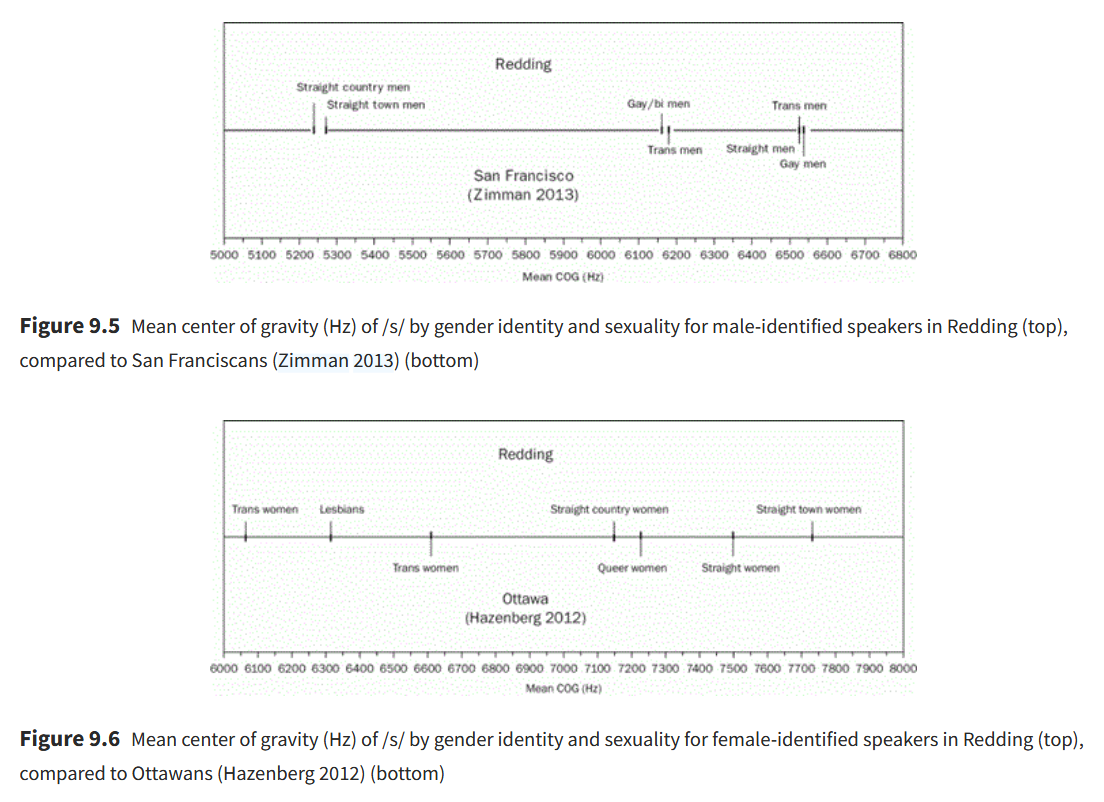
\includegraphics[width=\textwidth]{./images/podesva_sexuality_2016.png}
\caption{Spectrum of mean /s/ CoG by identity group from \textcite[p. 181]{podesva_sexuality_2015}, synthesizing with data from \textcite{hazenberg_language_2012, zimman_hegemonic_2013}.}
%TODO: recreate this visual so that it's easier to read, all in one single spectrum, and has all of hazenberg's data rather than just the women part of it!!
\label{figure_cog_spectrums}
\end{figure}

	Although \textcite{podesva_sexuality_2015, hazenberg_language_2012, zimman_hegemonic_2013} include white queer cisgender people and white binary transgender people alongside white cisgender heterosexual speakers, \textcite{calder_whose_2021} argues these spectra nonetheless paint a picture of cisgender heterosexual white norms. They note that the indexicalities that can be construed from these spectra reflect these norms-- /s/ frontness is construed as feminine, and /s/ backness is construed as masculine, since cisgender heterosexual men and women form the extremes of the /s/ frontness spectrum, and queer speakers are figured as deviant from these indexicalities. \textcite{calder_whose_2021} argues that this indexicality makes up the cisgender heterosexual white indexical field for /s/, and the judgments associated with it, by which /s/ pronunciations outside of the white cisgender heterosexual norm are viewed negatively as a failure to properly index one's gender, represent those of the cisgender heterosexual white listening subject.
	
	Research on cisgender, heterosexual white listeners sheds additional light on the structure, application, and boundaries of this indexical field. \textcite{strand_uncovering_1999} finds that when cisgender heterosexual white listeners are asked to categorize audio stimuli on a spectrum of /s/ frontness as either /s/ or /∫/ (the English `sh' sound, as in `shirt', which is similar to a very backed /s/), they place the boundary higher when told the speaker of the audio clip is a woman than when they are told it is a man, thus indicating an indexical link between /s/ frontness and womanhood/femininity. In men's voices, a number of studies find that fronted /s/ is perceived as gay by cisgender heterosexual white listeners (\cite{pharao_indexical_2014, maegaard_s_2015, levon_categories_2014, campbell-kibler_intersecting_2011}). \textcite{munson_influence_2006}, replicating Strand's experiment with a larger range of stimuli, find that when listeners perceive a speaker to be lesbian sounding, they place the boundary between /s/ or /∫/ lower, thus expecting lesbians to back /s/. These indicate an additional indexicality within the cisgender heterosexual white indexical field of /s/, in which if the combination of /s/ front/backness does not conform with the expectations of the speaker's perceived binary gender, this speaker will be perceived as gay/lesbian. 
	
	\textcite{jessee_cisgender_2025} run another replication of \textcite{strand_uncovering_1999}, comparing the placement of the boundary between /s/ and /∫/ when the perceiver is told the speaker is trans vs. not told they are trans (and thus is likely to assume that they are cis). They find that unlike in \textcite{munson_influence_2006}, where queer cisgender speakers are expected not to conform with the expected /s/ pronunciation for their gender, transgender speakers are expected to hyper-conform-- trans women are expected to front /s/ more than cis women by all listeners, and listeners who do not know a trans person also expect trans men to back /s/ more than cis men. Although indexicalities certainly would have changed in the 20 years between these studies, it is nonetheless surprising that cisgender heterosexual white listener holds different expectations and perceptions for trans people than for queer cisgender people, especially since it is counter to trans speakers' actual behavior; \textcite{podesva_sexuality_2015, hazenberg_language_2012} both find that trans speakers' /s/ pronunciations are less extremely gender-differentiated than cis speakers'. \textcite{jessee_cisgender_2025} analyze this through the lens of the cisgender listening subject, seeing that rather than basing perceptions on transgender speakers' actual speech, the cisgender listening subject places strict standards on transgender speakers to conform to the binary more than even cisgender speakers. 
	
	By `conform to the binary', here I mean to conform to the binary gender the trans speaker currently identifies with, rather than the gender that they were assigned at birth. If perceivers conceive of conformance with the binary to be conformance with the gender norms of a trans person's gender assigned at birth (rather than their actual, current gender), a different understanding emerges in which perceivers expect transgender people to be more deviant from that norm than queer cisgender people of that gender assigned at birth. It is important to note the epistemological disjuncture here; this mode of perceiving transgender speakers requires a rejection of their view of their own gender, in favor of the cis perceiver's view that one's gender is a static consequence of their bodily characteristics. Regardless of whether the perceivers expect trans speech to be highly deviant from their assigned gender at birth or highly conformant with their gender identity, the cisgender listening subject nonetheless construes real trans speakers as inadequately performing gender. Furthermore, this structure of meanings does not include a possibility of indexing a transgender identity using /s/. Trans speakers are `damned if they do, damned if they don't' -- if a trans woman does not front /s/, her transness may be questioned, and she may be heard as a man; if she fronts /s/, she may be construed only as a gay man, not a trans woman. In this way, the cisgender heterosexual white indexical field marginalizes transgender, nonbinary, and other non-cisgender people more than it does queer cisgender people. To avoid applying this marginalizing lens, research that has been conducted on non-cis, non-white speakers' /s/ productions has tended to simply get out of the cisgender listening subject's ears, so to speak, by studying the ways in which these communities forge new indexicalities of /s/ in interactions with other transgender people within local, community-oriented indexical fields.
	
	It is notable that two of the perception studies cited above -- \textcite{maegaard_s_2015, levon_categories_2014} -- already provide evidence that the indexical meanings of femininity and gayness for /s/ frontness were specific to the cisgender heterosexual white indexical field, and that other indexical fields may exist. \textcite{maegaard_s_2015} finds that listeners in Copenhagen only hear fronted /s/ as feminine and gay when it is within the context of standard Copenhagen Danish speech, and do not hear it as these things when situated in a locally-present speech style known as `street' speech, as this speech style also happens to feature fronted /s/ and is associated with immigrants, `gangster'-ness, and masculinity. Although Maegaard and Pharao do not use indexical fields in their analysis, this would nonetheless be an example of a meaning of /s/ within a local indexical field taking precedence over the hegemonic indexical field within a non-white context. \textcite{levon_categories_2014} finds that indexicalities within the hegemonic indexical field also are limited to listeners who hold hegemonic attitudes; those who endorse normative masculinity and male gender roles perceived fronter /s/ to be more feminine and gay, whereas those who reject these attitudes do not make these indexical connections. From these studies, it is clear that the construal of fronted /s/ as indexical of femininity and gayness is associated with a white, cisgender, heterosexual, and gender-normative judgmental listening subject, and situated within the corresponding indexical field (as pointed out by \cite{calder_whose_2021}), and that other indexicalities and listening subject positions exist. Recent research on trans and non-white speakers' usage of /s/ takes a closer look at these alternative indexical fields and investigates how these indexicalities come about.
	
	\textcite{calder_sissy_2019} applies the theories of indexical orders developed by Silverstein \parencite*{silverstein_language_2023, silverstein_indexical_2003}, and fractal recursivity developed by \textcite{irvine_language_2000, gal_boundaries_1995} in order to investigate this process. As linguistic forms are construed as indexical signs and gain meaning within a particular indexical field, it is possible that new meanings will arise which build off of and are informed by the original meaning. This can take place both within a single indexical field, and cross-cutting the overlaps of multiple. The development of an indexical link between a linguistic form and a social meaning always already emerges informed by an uncountable chain of previous semiotics, and for this reason is said to exist at the $n$th indexical order (\cite{silverstein_indexical_2003}). In the case of /s/, Calder understands the indexical link between the gender binary and /s/ frontness to exist at the $n$th order within the hegemonic indexical field. When cisgender heterosexual white listeners' perception of a speakers' gender does not match with their perception of that speaker's /s/ pronunciation, this recontextualization of /s/ usage forms the $n + 1$st indexical order, by which speakers are held to be indexing gender nonconformance. At this point, the epistemological disjuncture mentioned above once again rears its head; Calder's model assumes that cisgender listeners enforce the norms of /s/ based on their perception of the speaker's assigned gender at birth, erasing transgender, nonbinary, and other queer identities and subsuming all gender nonconformance as gay/lesbian. In this way, the $n + 1$st order indexicality of /s/ front/backness becomes gay/lesbianness, rather than simply gender nonconformance. It is important to note that although the $n$th and $n + 1$st indexicalities of /s/ are situated at different orders, they nonetheless inform and construct each other, and do not form a chronological order despite their ordered structure. 
	
	Within the San Francisco drag communities \textcite{calder_sissy_2019} studies, an additional indexical order of /s/ is forged at the $n + 1 + 1$nd level which is local to these communities' indexical fields, escaping the hegemonic field. A drag community Calder studies in the South of Market (SoMa) neighborhood of San Fransisco figures itself as more radically queer than another drag community they study in the Castro neighborhood. This is reflected by the differences in identities between these communities; SoMa queens generally identify as non-cisgender and challenging to the gender binary, many of them nonbinary or transgender, whereas the queens of the Castro neighborhood primarily identify as cisgender gay men. Calder finds that SoMa queens front /s/ more than Castro queens, and that this forges a new local indexicality to `fierceness', deviance from gender norms, and and in-group status at the at the $n + 1 + 1$nd level. Their diagram of this structure of meanings is included in figure \ref{figure_fractal_recursivity_indexical_orders}. This emerges as an example of indexical orders cross-cutting indexical fields, where meanings in the hegemonic cisgender heterosexual white indexical field came to inform the creation of new meanings in the local, alternative indexical field.

	It was mentioned above that within Calder's model, fronting /s/ emerges as deviant from gender norms only in those whose gender is understood as `male' within the cisgender, transphobic conception of gender as bodily characteristics. It is perhaps surprising, then, that nonbinary and transfeminine speakers in the SoMa drag community, who would likely be gendered this way, front /s/ exactly for the purpose of gender deviance, rather than gender conformance. It is helpful to introduce a theoretical tool Calder employs to understand the interlinking of identity categories at these different levels of sex at birth, gender identity, sexuality, and trans/queerness-- the semiotic process of fractal recursivity, as theorized by \textcite{irvine_language_2000, gal_boundaries_1995}.
	
	In fractal recursitivity, a semiotic opposition on one level becomes nested into itself, and this process can happen any number of times (\cite{irvine_language_2000, gal_boundaries_1995}). In the first two indexical orders of /s/, both of which are within the cisgender heterosexual hegemonic white indexical field, the gender binary is nested into itself, creating a metaphorical structure where men are split into a binary gender opposition. This can be understood as distinguishing some notion of `men who are men' from `men who are women', and `women who are women' from `women who are men'. These become the metaphorical representation of gay men and lesbian women, since members of these groups are still fundamentally understood as types of men and types of women, rather than something else entirely, as with transgender and nonbinary people. Is it then the case that by situating the distinction between cisgender gay Castro queens and nonbinary and transgender queer SoMa queens as nesting into the `men who are women' branch, Calder as the analyst, and possibly the drag queens themselves, tacitly consider these queens as nonetheless a `type of man/male'? I argue it is not. Instead, in my reading of Calder's work, SoMa queens reinterpret the binary distinction at the $n + 1$st level, instead of as gay cisgender men vs. straight cisgender men, as gay men vs. queer non-cisgender people, or as Calder articulates it, gay vs. queer. This binary still fits into the structure, as it is not difficult for SoMa queens to figure gay men as less feminine and less subversive than queer non-cisgender people. From here, the indexicality of /s/ frontness as subversive queer non-cis femininity can be less problematically interpreted.
	
\begin{figure}[h]
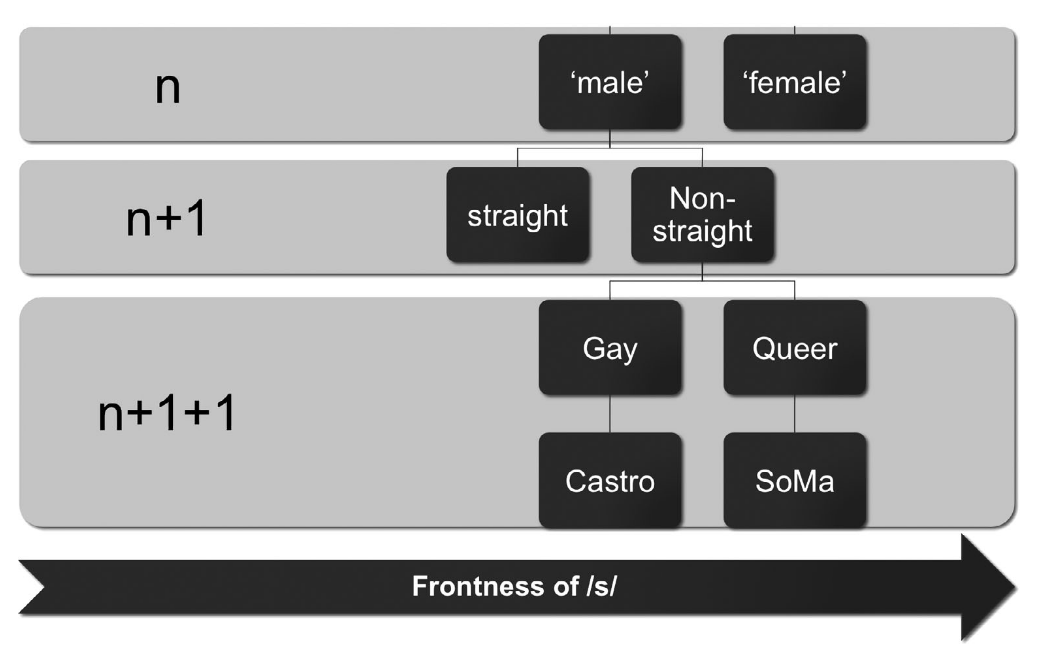
\includegraphics[width=\textwidth]{./images/calder_sissy_2019_fig6.png}
\caption{Diagram from \textcite[p. 340]{calder_sissy_2019} illustrating indexical orders of /s/ frontness and corresponding fractal recursive social oppositions across two San Fransisco drag communities.}
\label{figure_fractal_recursivity_indexical_orders}
\end{figure}

It is also not necessarily the case that alternative meanings of /s/ emerge through this sort of fractal-recursive process. In some cases, speakers more directly contradict hegemonic meaning structures rather than subversively repurposing and reinterpreting them. For example, \textcite{steele_enacting_2022} investigates a community of Columbus, Ohio nonbinary individuals, and finds that not only did speakers' rating of their identification with masculinity not correlate strongly with /s/ backness among white speakers, but that this rating had a positive correlation with /s/ frontness among non-white speakers. This behavior suggests an indexicality within this Columbus nonbinary indexical field which is the inverse of that of the hegemonic indexical field at a higher indexical order. Similarly, in Bakersfield, California,  \textcite{calder_whose_2022} find that cisgender heterosexual Black speakers were not significantly different in /s/ frontness with respect to gender. In this case, the Bakersfieldian Black indexical field may associate gendered /s/ pronunciations with whiteness; this meaning could also be understood to emerge at a higher indexical order, forged through the situation of the hegemonic meaning into its racial context. 

The studies discussed above illustrate the ability of speakers outside of cisgender white heterosexual populations to construct alternative and subversive meaning structures for /s/ which allow an interpretation of their unique speech practices as innovative and subversive rather than inadequate and deviant. However, due to the dominance of the hegemonic indexical field, and the practicalities of social life, it is nonetheless the case that those of us outside of cisgender white heterosexual populations have to interact with people within these populations who may inhabit the associated listening subject position and make these negative judgments of our speech. In this situation of indexical misalignment, in which speaker and listener have differing indexical inventories, it is marginalized speakers who are expected to adapt, as privileged listeners will entitle themselves to the universal application of their indexical inventory. As mentioned above, a speaker in \textcite{heffernan_constructing_2023} notes that she modifies her voice when interacting with the `cis universe'. Drawing upon all of this prior work on indexicalities of /s/, this thesis investigates whether this sort of modulation involves /s/, and the implications and indexicalities that arise through the transfeminine speakers' behavior within the specific situation of indexical misalignment.

That individuals may change their /s/ pronunciations within interaction for gender-presentational and interactional purposes has been attested by \textcite{benesch_stylizing_2022, mendoza_that_2024, saigusa_jane_2016, holmes-elliott_substance_2017, levon_east_2013, parnell-mooney_transgender_2019, calder_fierceness_2019, zimman_variability_2017}. \textcite{holmes-elliott_substance_2017, levon_east_2013}, in a study of within-speaker variation in /s/ pronunciation in British reality television shows, find that in one lower-class show, cisgender heterosexual women use backer /s/ in conversation with other women, whereas in a higher-class show, cisgender heterosexual women use fronter /s/ in this context. In order to explain these contradictory results, they conclude that the interlocutor's gender may not be the best predictor, as in both shows women back /s/ in speech activities considered more threatening. As discussed below in the methods chapter, the recorded conversations I conducted attempted to control for this stance-based shifting through the structure of two collaborative-valenced speech activities.

Moving to investigate /s/ shifting in queer speakers, \textcite{calder_fierceness_2019} finds that as SoMa drag queens get into their drag, visually transforming into their drag persona, their /s/ pronunciations get progressively fronter to index their change in persona. \textcite{benesch_stylizing_2022} finds that among genderfluid people, who experience different genders at different times, shifts in /s/ index these shifts in gender, however they do not necessarily correlate with typical scales of gender such as masculinity vs. femininity, but rather with personal, alternative scales such as `flannel' vs. `glitter'. In a case study of a Latinx  drag queen part of a drag community in Wynwood, Miami who exhibited particularly wide variation in /s/ pronunciations, \textcite{mendoza_that_2024} finds this queen uses fronter /s/ when discussing the aspects of their drag taken from white, higher-class femininity, but uses backer /s/ when aligning themself to the more anti-normative parts of their \textit{chonga} drag persona, where \textit{chonga} is a queer subversive Latinx femininity which may look like ``unshaved body hair and beards, as well as hoop earrings and dramatic lip liner'' (307). The polyvalence of this queen's drag persona is indexed through these changes in /s/. Specifically of note here is that for them, fronted /s/ is not indexical of femininity in general, but rather indexical of a specific white cisgender heterosexual higher-class femininity. In this way, meanings are reinterpreted in order to subvert the white cisgender listening subject. 

I choose to focus on /s/ rather than other linguistic forms bearing social indexicalities because of the theoretical depth of the research that has already been conducted on /s/; this research has captured a nuanced and detailed view of the hegemonic indexical field of /s/, how it is marginalizing, and how those who are marginalized by it reinterpret and construct its meanings subversively within their communities. However, in the /s/ literature, as well as in sociolinguistic research more broadly, a gap I address is the dearth of research looking specifically at situations of conflicting indexical fields, analyzing how interactions play out between individuals with different indexical inventories. Comparing transfeminine individuals' /s/ pronunciations in conversations with another transfem, where they can adopt their own indexicalities more freely, against their /s/ pronunciations in conversations with a cis woman, is illuminating here. More broadly, this research also addresses the absence of intra-speaker research on transfeminine speakers-- although there have been  of studies of intra-speaker variation in transmasculine people (eg. \cite{zimman_variability_2017, parnell-mooney_transgender_2019}), nonbinary people (\cite{gratton_resisting_2016}), and drag queens (\cite{calder_fierceness_2019, mendoza_that_2024}), there have been no such studies focused on how transfeminine speakers speak differently in differing situations. A final question my study hopes to address is to understand how transfeminine individuals navigate the trans-exclusive fractal-recursive indexical orders of /s/ indexicality, as developed by \textcite{calder_sissy_2019} and discussed above, when forging new indexicalities may not be recognized or well-received by a cisgender listener. This thesis thus pursues the research question:
\begin{quote}
Do transfeminine speakers shift towards fronter /s/ pronunciations with a cis woman listener versus with a trans woman listener? What factors determine this choice?
\end{quote}

Based on the literature reviewed, I predict:
\begin{enumerate}
\item Speakers who express greater feelings of danger, discomfort, dysphoria, or desire to pass around cisgender people are more likely to shift;
\item Speakers who differentiate themselves from or hold attitudes of resistance against hegemonic femininity are less likely to shift;
\item and Speakers who express concern with gay-male misrecognition are less likely to shift.
\end{enumerate}
These predictions are primarily based on the structure of the indexicality /s/ within the hegemonic indexical field. Because of transfeminine people's awareness of the cisgender listening subject's application of hegemonic norms, I expect that transfeminine speakers' decision making around /s/ shifting will be based upon their relationship with the meanings of /s/ in the hegemonic field, as well as their relationship with hegemonic feminine norms itself; if speakers wish to distance themselves from hegemonic femininity, they will not take up a fronter /s/ because they will not be interested in hegemonically indexing femininity. However, if speakers feel greater pressure to conform to hegemonic femininity, they are likely to shift towards fronter /s/ pronunciations in self-defense and to match up to the hegemonic standards. Yet, if speakers are concerned with being mistaken for a gay man via their voice, they may feel that even if they would be able to benefit from indexing hegemonic femininity, that /s/ is not an available resource through which to do so.

% First, as discussed above, transfeminine people may choose not to front /s/ with cisgender listeners to avoid misrecognition; they may guess that their listener is more likely to misrecognize a fronted /s/ as indexing a gay man identity (using the $n + 1$st indexical order), rather than a feminine one (at the $n$th). Second, shifting towards a more normative index is a mechanism of defense, and some transfeminine speakers may feel less of a need to defend themselves. This situation again has two possible arrangements. First, some speakers may feel less threatened by cisgender listeners than others, perhaps due to non-linguistic factors such as the communities they are in or confidence that they will be gendered correctly regardless of their voice. Second, some speakers may choose not to shift /s/ as a move of resistance, simply refusing to bend towards cisgender norms and cater to cisgender judgements.

% Through the process of my interviews with participants, I aim to discover speakers' attitudes and experiences with their voices and existence in the cisgender world. I predict that these attitudes and experiences will align with linguistic behavior, supporting an agentic view of transgender people's language use.

% I predict that speakers will not shift /s/ in three possible cases:

% However, if a speaker primarily expresses concern with being misgendered and places importance on ``passing'', I predict they will shift in order to achieve these goals.

% \section{extra stuff}

% \textcite{zimman_hegemonic_2013} finds that a group of cisgender, majority-heterosexual listeners rated cis gay voices and trans men's voices as similarly gay-sounding, despite differences in these groups' language use: trans men's /s/ pronunciations were significantly lower in CoG than cis gay men's and significantly higher in skewness. He concludes that in judging gay-soundingness, percievers do not listen for a single linguistic feature or set of features but instead judge deviance from cisgender hegemonic masculine speech across many linguistic features.

% \textcite{zimman_}

\chapter{Methodology}

In order to investigate whether and how transfeminine individuals change their pronunciations of /s/ based on the trans status of their conversation partner, and to be able to interpret the possible motivations behind these patterns of change, I recruited four transfeminine individuals to be speakers and two women, one cisgender and one transgender, to be conversation partners (CPs). Each speaker participated in an audio-recorded, semi-structured casual conversation session with the each of the conversation partners, then completed a demographic survey, then participated in an audio-recorded semi-structured interview with me about their transgender experience and their relationship with their voice. This order of study activities was selected to minimize priming effects, since it is possible questions asked in the survey and interview could effect subsequent linguistic behavior.

\section{Participants}
All participants were students of Reed College between the ages of 18 and 25, recruited by flyers, word-of-mouth, and email. All speakers identified as transfeminine, and both conversation partners identified as women; one identified as cisgender and one identified as transgender. Speakers are referred to by animal-name pseudonyms, and the conversation partners are referred to as `the Cis CP and `the Trans CP' respectively.

\subsection{Survey}
On the survey, participants were asked to provide any and all gender, sexuality, and race labels they identify with, as well as their pronouns. With respect to gender identity, I additionally asked participants to rank on the survey how much they generally identify with femininity and masculinity on scales of 0 to 100. However, I decided not to make use of the responses for these questions, as most of the participants seemed to find them uncomfortable and difficult to answer meaningfully. For the participants who were not the Cis CP, the survey also asked whether the participant was currently on hormone replacement therapy (HRT) and for how long they had been on it, whether they had received voice feminization therapy and whether they had received voice feminization surgery. All of the trans participants were on HRT, and no participants had received voice feminization therapy or voice feminization surgery. Questions were also included to understand speakers' linguistic backgrounds-- what languages they speak, whether they have primarily spoken English throughout their life or have had periods of primarily speaking other languages, the region(s) in which they grew up, and whether they had received non-gender-related speech therapy. Survey questions are provided in appendix \ref{appendix_a}.

\subsection{Interviews}
%TODO: go through the interviews and transcribe all of the questions i asked
After conversation sessions and surveys were completed, I also conducted 20-30 minute audio-recorded semi-structured interviews with the speakers. As a starting point, I asked questions intended to elicit background on each participant's individual relationship and history with gender and sexuality beyond the labels collected in the survey. From here, I hoped to see how participants position themselves with hegemonic femininity, and how this relationship may have changed and developed over the course of transition. The discussion that followed from these questions tended also to address the question of `outness'; what this meant for each speaker, and how private their trans and queer status was. After this, I moved to asking questions about participants' relationships with their voices. Some of these questions were modeled after those used by \textcite{heffernan_constructing_2023} to investigate speakers' understandings of the cisgender listening subject, asking speakers to talk about how they feel their voice is perceived by cis listeners and whether they might speak differently around different people. I did not directly ask speakers whether they were concerned that their voice would be mistaken as a gay man's voice, instead allowing the topic to naturally arise if it was salient to the participant. I also included in this portion questions about sexuality and the voice, such as ``Do you feel that your voice sounds lesbian?'', in order to get a sense of the relationship sexuality may play in determining /s/ pronunciation and shifting behavior. A full list of questions is provided in appendix \ref{appendix_b}. Participants' demographic information and gender background from survey responses and interviews are summarized in tables \ref{demographics} and \ref{gender_backgrounds}.

\begin{table}[h]
\begin{small}
\begin{tabular}{l p{3cm} p{3.2cm} p{2.2cm} p{1.8cm}} \toprule
Participant & Gender & Sexuality / \newline Prefers to Date & Race & First \newline Language \\
\midrule
Mantis \textsuperscript{(she/her)} & (Trans) Woman, \newline (Trans) Girl & Queer; \newline Trans men,  \newline Nonbinary People& East Asian, \newline Taiwanese, \newline Japanese, \newline Wasian & English \\
Alpaca \textsuperscript{(she/it)} &  Woman, Girl & Lesbian & White & English \\
Squirrel \textsuperscript{(she/her)} &  Transfem, \newline Trans Girl & Bisexual; \newline Fem People & White & English \\
Jellyfish \textsuperscript{(she/her)} &  Woman & Lesbian & White & English \\
Trans CP \textsuperscript{(she/her)} &  Woman & Ace spectrum, \newline Demisexual & East Asian, \newline Han Chinese & Mandarin\\
Cis CP \textsuperscript{(she/her)} & Woman & Lesbian & white & English\\
\bottomrule
\end{tabular}
\end{small}
\label{demographics}
\caption{Participants' Demographic Identity Information, from survey and interviews}
\end{table}

\begin{table}[h]
\centering
\begin{small}
\begin{tabular}{l l l} \toprule
Participant & Time Out & Time on HRT  \\
\midrule
Mantis & \textasciitilde3yr & 1y8mo \\
Alpaca &  \textasciitilde4yr & 3yr9mo \\
Squirrel & 9mo (primarily online) & 3mo \\
Jellyfish & >3yr & \textasciitilde2yr \\
Trans CP & 4yr & 3yr \\
\bottomrule
\end{tabular}
\end{small}
\label{gender_backgrounds}
\caption{Participants' Transgender Background Information, from survey and interviews}
\end{table}

\section{Conversations}
Before the survey and interviews, speakers participated in two 20-30 minute audio-recorded conversation sessions, one with each of the conversation partners. As these recordings would be subject to acoustic analysis of /s/, they were conducted in a sound-isolated recording booth using clip-on lavalier microphones (on the speaker as well as the conversation partner) connected to a Zoom h4n recorder. Participants were told to spend the first 10 minutes of the recording time collaboratively playing a word game of their choice (crossword, New York Times Wordle, New York Times Connections, etc.). This prompting was intended to get participants comfortable talking with each other on the recording and to take up a collaborative and friendly stance towards one another. Controlling for stance in this way was intended to isolate stance-related variation in /s/, as indexicalities between /s/ and confrontational/threatening stances have been found (see \textcite{holmes-elliott_substance_2017}). Speakers and CPs were asked to time themselves and stop playing the game after the first 10 minutes of the recording, and to spend the rest of the time of the recording, another 15-20 minutes, getting to know each other, trying to find things in common, and talking about shared experiences. Since Alpaca and the Trans CP told me that they already knew each other, they were asked to catch up and chat as they would normally. The rest of the speakers and conversation partners did not know each other. The second portion of the conversation was intended to elicit free-flowing casual talk with a similarly friendly and comfortable stance orientation.

\section{Analytical Approach} \label{analytical_approach}
In order to answer the first portion of my research question, whether transfeminine speakers shift towards fronter /s/ pronunciations with a cis woman listener versus with a trans woman listener, I take a quantitative empirical approach. I operationalize spectral center of gravity (CoG) of /s/, measured in Hz, as the dependent variable, and conversation partner (Cis CP vs. Trans CP) as the independent variable. In order to measure CoG of /s/, I produced a time-aligned plain-English transcript of each recording. As a first pass, I used Deepgram's Nova 3 speech recognition model, specifying that it should transcribe utterances (rather than paragraphs or unsegmented) and annotate each utterance with who it was spoken by: the speaker or the conversation partner. I then used a Python script to convert the output of this model into a time-aligned transcription file format (TextGrid) usable by the linguistic acoustic analysis software Praat (\cite{boersma_praat_2023}). I then used Praat to manually correct the transcripts to ensure accuracy. I then used the Montreal Forced Aligner with the included English acoustic model and dictionary to automate the production of a time-aligned phonetic transcript, which would specify, for both the speaker and the conversation partner, the start and end time in the recording of each /s/ pronunciation \cite{forced_aligner}. From there, I used DiCanio's \parencite*{dicanio_spectral_2021} Praat script to measure the CoG of each of these /s/ pronunciations in each of the recordings for the speakers and conversation partners. It was important to measure not only the /s/ pronunciations produced by the speaker participants, but also those produced by the conversation partner participants, in order to determine the extent to which the speakers may have been responding to the /s/ pronunciations of the conversation partners (and vice versa). I used the statistical analysis software R (\cite{r_core_team_r_2025}) to combine, statistically analyze, and visualize the data.

In determining the second half of my research question -- what factors determine the choice to shift vs. not shift to a fronter /s/ pronunciation with the Cis CP -- I take a qualitative approach. I use interview responses to qualitatively assess the extent to which each speaker aligns with the three criteria in my predictions, quoting and discussing instances in which speakers:
\begin{enumerate}
 \item express feelings of danger, discomfort, dysphoria, or desire to pass around cisgender people;
 \item differentiate themselves from or hold attitudes of resistance against hegemonic femininity;
 \item and express concern with gay-male misrecognition.
\end{enumerate}
This approach is intended to encourage my analysis of speakers on their own terms, rather than simply comparing them against a white cisgender heteronormative standard which will inevitably find them somehow faulty (see \cite{calder_interrogating_2025, zimman_beyond_2021}). Instead, I aim to understand the connections between speakers understandings of their voices and their vocal behavior, underlining instances of strategic deployment of semiotic resources, as well as the oppressive limitations imposed by cisnormativity.

\chapter{Results}
\begin{table}[h]
\centering
\begin{tabular}{l r r r r}
\toprule
		  & \multicolumn{2}{c}{Number of /s/ tokens}  &  \multicolumn{2}{c}{Duration of Recording}\\\cmidrule(r){2-3} \cmidrule(r){4-5}
Speaker & w/ Trans CP & w/ Cis CP & w/ Trans CP & w/ Cis CP \\ \midrule
Mantis    &       177 &       143 &       21m48s &     14m31s \\
Alpaca    &       476 &       244 &       30m56s &     21m53s \\
Squirrel  &       388 &       401 &       25m04s &     29m49s \\
Jellyfish &       444 &       283 &       26m27s &     20m08s \\
 \bottomrule
\end{tabular}
\caption{Table of number of /s/ tokens measured and duration of each recording.}
\label{table_recordings}
\end{table}

\begin{table}[h]
\centering
\begin{tabular}{l r r r S}
\toprule
		  & \multicolumn{3}{c}{Mean /s/ CoG (Hz)}  &  \\\cmidrule(r){2-4}
Participant   & Overall & w/ Trans CP & w/ Cis CP & {$p$-value} \\ \midrule
Mantis    &    7231 &                   6638 &                7964 & < 0.001\\
Alpaca    &    5758 &                   5899 &                5483 & < 0.001\\
Squirrel  &    6357 &                   6345 &                6369 &   0.8263\\
Jellyfish &    6154 &                   6039 &                6334 & < 0.01\\
Trans CP  &    5133 &					N/A	 &				N/A    & N/A \\
Cis CP    &    6835 &					N/A	 &				N/A   & N/A \\
 \bottomrule
\end{tabular}
\caption{Table of Mean /s/ CoG used by each speaker, overall as well as separated by conversation partner (CP). $p$-value indicates the likelihood that the difference in means between Trans and Cis conversation partner could be a result of random chance; $p$-values of <0.01 indicate a statistically significant difference in means.}
\label{overall_table}
\end{table}

\begin{figure}[h]
	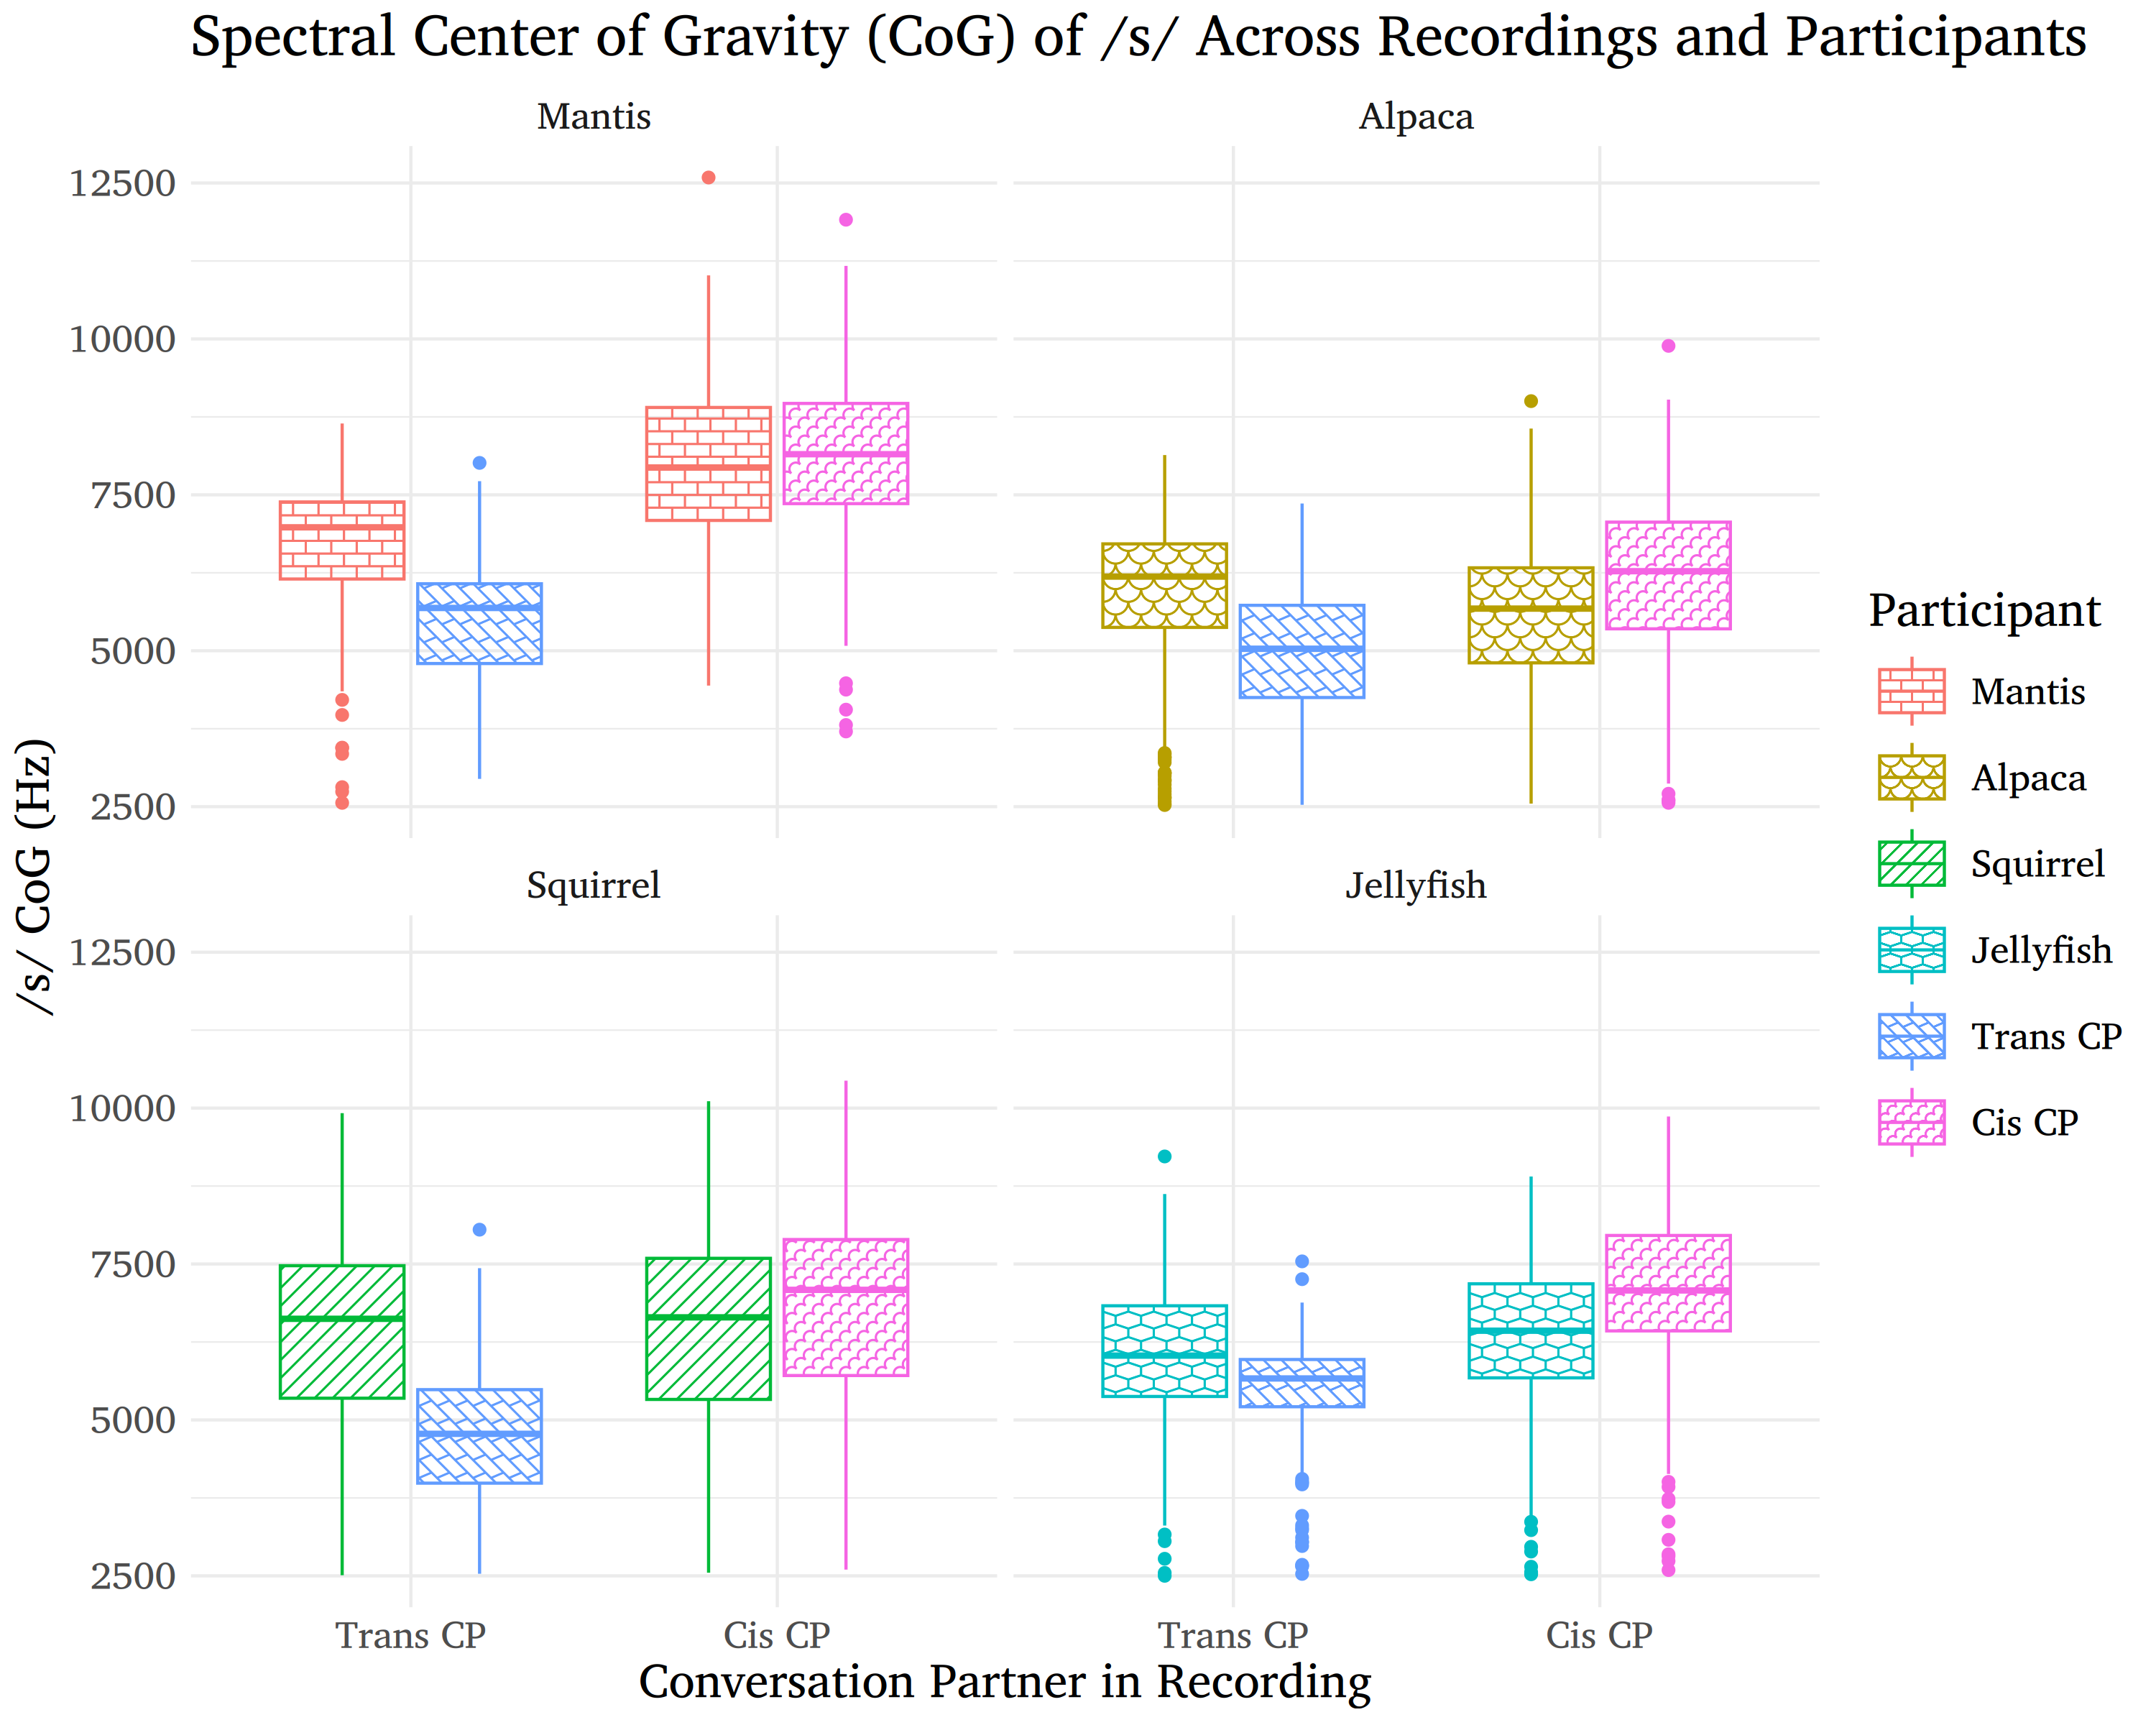
\includegraphics[width=\textwidth]{./images/overall_plot.png}
	\caption{CoG of /s/ pronunciations in each recording, by each speaker. }
	\label{overall_plot}
\end{figure}

Table \ref{table_recordings} lists the duration of each recording and the number of /s/ tokens produced by the speaker participant in each recording. Table \ref{overall_table} and figure \ref{overall_plot} present an overview of participants' /s/ pronunciations. \textcite{zimman_variability_2017} reports that so-called `reference' studies on white English speakers presumed to be cisgender and heterosexual report a `typical' /s/ CoG range of 6,400Hz--8,500Hz for women and 4,000--7,000Hz for men. That only Mantis and the Cis conversation partner fell inside this range expected of women, and that only Mantis fell outside this range expected of men, points towards the inadequacy of these `reference' values outside the hegemonic field (recall that the Cis CP is a lesbian). I argue that this discrepancy should not be read as an indication of inaccurate or flawed measurement methodology, however, as these means used by my speakers do align with previous measurements for queer and trans women: the white trans women and cis lesbians \textcite{podesva_sexuality_2015} study in Redding, California exhibit mean /s/ CoG ~6,000Hz and ~6,350Hz respectively, and the white trans women \textcite{hazenberg_language_2012} studies in Ottawa, Ontario exhibit a mean /s/ CoG of ~6,600Hz. These measures align much more closely with my speakers, with the exception of the Trans CP and Mantis, who occupy the extremes of my data. I will return to these individual cases, but for now it is sufficient to consider the general correspondence of my data with previous studies of trans and queer women to attest to my data's validity.

With respect to shifting, three of my four speakers exhibit statistically significant differences in /s/ pronunciation between the recording in which they spoke with the Trans CP and the recording in which they spoke with the Cis CP, and one speaker, Squirrel, did not. Of the three speakers who shifted, two, Mantis and Jellyfish, shifted in the direction of fronter /s/ pronunciations producing higher CoGs when talking to the Cis CP, coming into closer alignment with hegemonic expectations of the feminine voice; the other speaker, Alpaca, shifted in the opposite direction, using more hegemonically-feminine /s/ pronunciations with the Trans CP. With respect to the degree of shifting, Mantis exhibited the largest shift with a difference in means of >1000Hz, while Alpaca and Jellyfish shifted more subtly.

In the sections that follow, I consider each speaker's behavior individually and perform the qualitative assessments of the attitudinal factors listed above in section \ref{analytical_approach}. I attempt to explain speakers' /s/ pronunciations in comparison to prior literature, my understanding of their identity and background, and these attitudinal factors. Following this, chapter 4 consists of a synthesis of these analyses, and a discussion of the implications of this data for the theories and research questions presented in chapter 1.

\section{Speaker 1: Mantis}
\begin{figure}[h]
	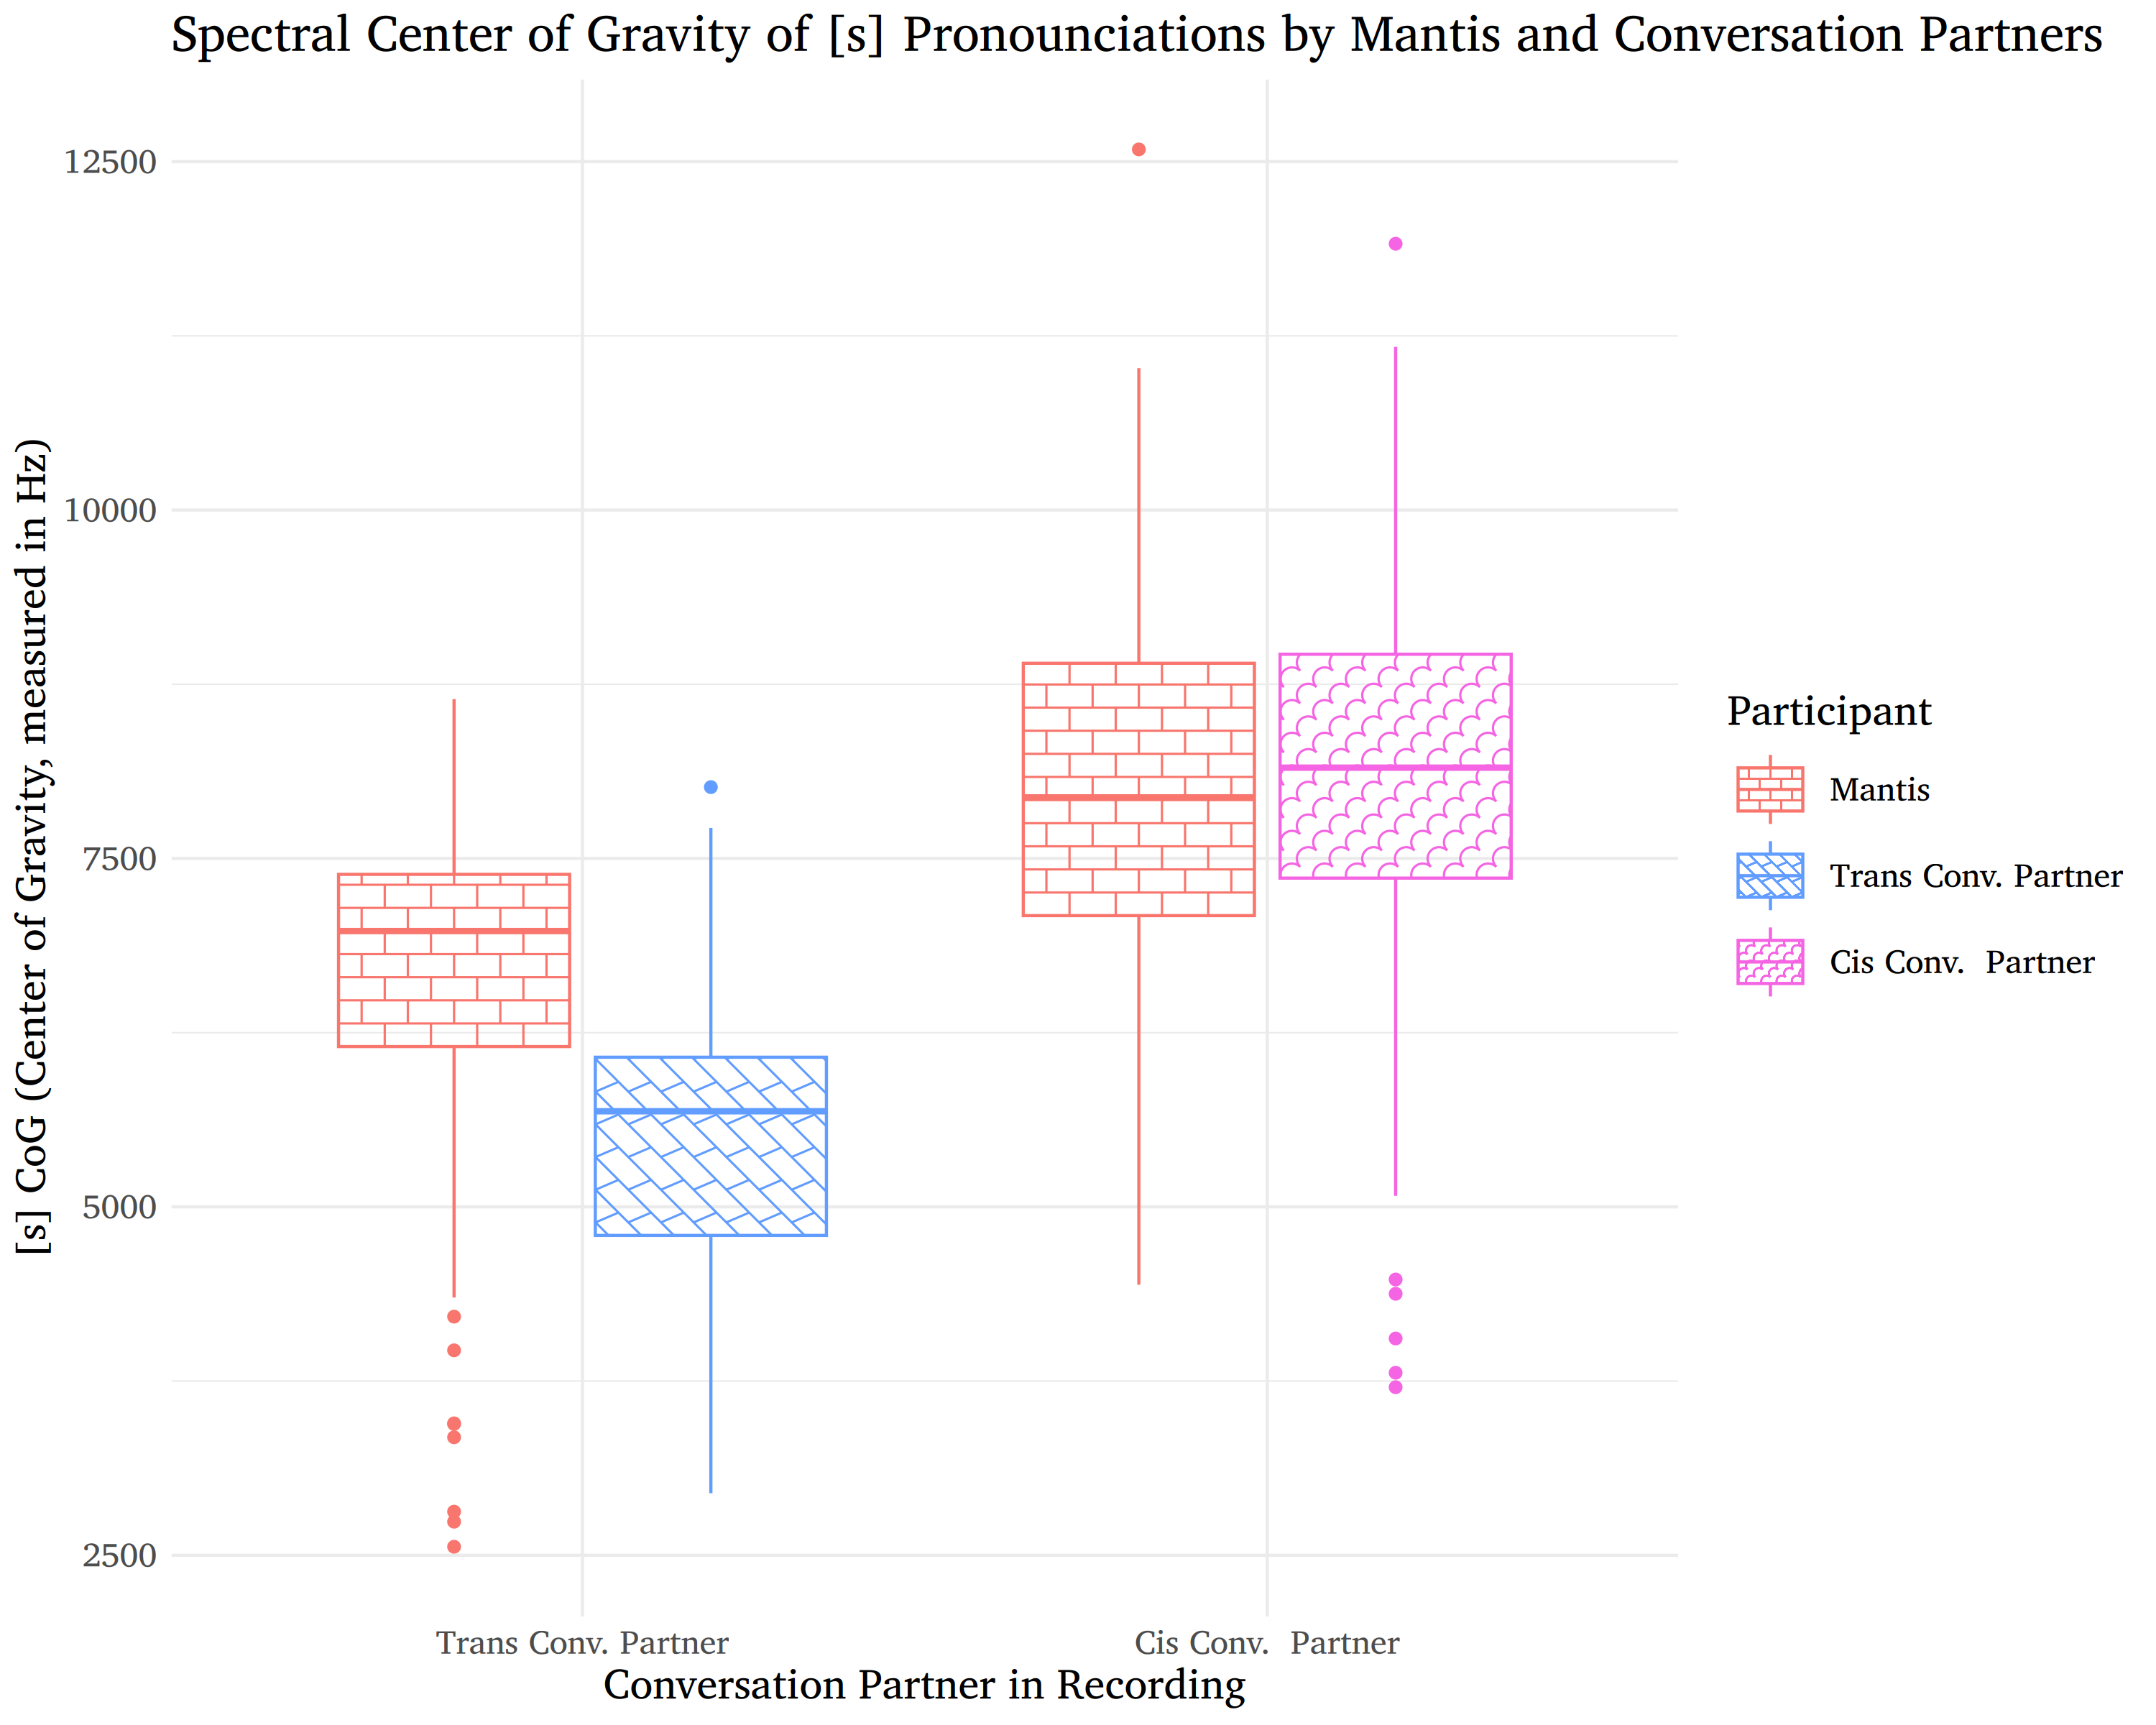
\includegraphics[width=\textwidth]{./images/Mantis _plot.png}
	\caption{CoG of /s/ pronunciations in each recording containing Mantis, her pronunciations and the pronunciations of the conversation partners.}
	\label{mantis_plot}
\end{figure}

Figure \ref{mantis_plot} zooms in on Mantis' /s/ pronunciations. Her /s/ pronunciations are distinct from the other speakers' not only because her shift is the largest, but also because her overall mean CoG, regardless of conversation partner, is also the highest. As mentioned above, her /s/ pronunciations fall within the hegemonically-expected `reference' range for cisgender women with an overall mean of 7231hz. In my interview with her, Mantis told me that she has ``had so many people come and tell [her] that they thought [she] was a cis woman with [her] voice''; it is possible that her /s/ pitch contributes to these perceptions. She notes that these instances of having a cisgender-passing voice are the reason that she ``used to worry a lot about [her] voice, but now it doesn't bother [her] as much.'' Here, she constructs a narrative about the development of gender confidence over the course of transition. Alpaca, Jellyfish, and the Trans Conversation Partner -- the other participants in the study who had been out as trans women for multiple years -- all related similar stories of development in my interviews with them. Although this is somewhat expected as a part of a successful gender transition, it is nonetheless important to note, because this narrative often included the development of a greater comfort with deviation from normative standards of femininity. Mantis notes:
\begin{quote}
 ``I don't necessarily consider myself to be a woman in a way that a binary woman is a woman, but I also don't say I'm nonbinary, because I very much am like 100\% woman, it's just, not in anybody else's way.''
\end{quote}
These narratives strike me as constructing a stance of resistance against the norms of unitary hegemonic femininity; in understanding her womanhood as unique to her, Mantis asserts that she does not have to adhere to `anybody else's way' in order to be `100\% woman'. Here, Mantis provides a counter-example to one of my predictions, showing that stances of resistance and differentiation towards cisgender norms do not necessarily correspond with a refusal to shift towards those norms in interaction with a cisgender listener.

An additional counter-example provided by Mantis relates to the issue of misrecognition. She does attest that sounding like a gay man is a concern, but this does not lead her to avoid fronter /s/ pronunciations with the cisgender listener as I would have predicted. When asked about how her experience with her own voice has developed over time, she began her answer by noting that she has ``always had like `gay voice' or like feminine voice''. When I asked whether her voice dysphoria was the simple concern of not sounding feminine enough, she replied:
\begin{quote}
 ``... it was, more specifically, like `oh I just sound like a gay man'. And then there would be gay men who have gay voice ... and I'd be like 'oh I can't distinguish my voice from theirs', and it's just very frustrating, and I don't want people to think like that of me.''
\end{quote}
From this answer, it was clear that concerns about misrecognition represent an primary portion of Mantis's relationship with her voice. Although I will discuss the possible interpretations of this apparent mismatch in attitude and behavior later, for now it is sufficient to note that Mantis stands here as a counterexample to my prediction that speakers more concerned with misrecognition as a gay man would avoid fronter /s/ pronunciations with the Cis CP.

On the other hand, Mantis did provide evidence to support another of my predictions, the prediction that speakers who reported greater pressure to conform or `pass' with their voice in the presence of cisgender listeners would be more likely to shift to a fronter /s/ pronunciation with the Cis CP. In our discussion of voice dysphoria, Mantis mentions:
\begin{quote}
 ``in conference sometimes ... I'm like, I don't know, maybe I shouldn't speak, because the person who just spoke before me just sounded like, so, woman, and now if I speak, people are gonna think I sound like a man. ... especially with cishet women ... it’s almost like a competition."
\end{quote}
In these moments, Mantis feels that cisgender women's speech becomes the standard for feminine speech, and that the differences between her voice and the voices of cis women around her mark her speech as deficient and male. In order for feminine speech to be a `competition', not only does there have to be a unitary way to `win' -- the cisgender norm -- but further, she and her listener both have to make effort to change their speech towards this norm. And this is backed up in her behavior, as well as the behavior of the Cis CP; both of them shift towards fronter /s/ pronunciations. Not only does Mantis front /s/ much more than she did with the Trans CP, but the Cis CP's /s/ pronunciations were the frontest mean CoG when talking with Mantis (in comparison to the other speakers).

\section{Speaker 4: Jellyfish}
\begin{figure}[h]
	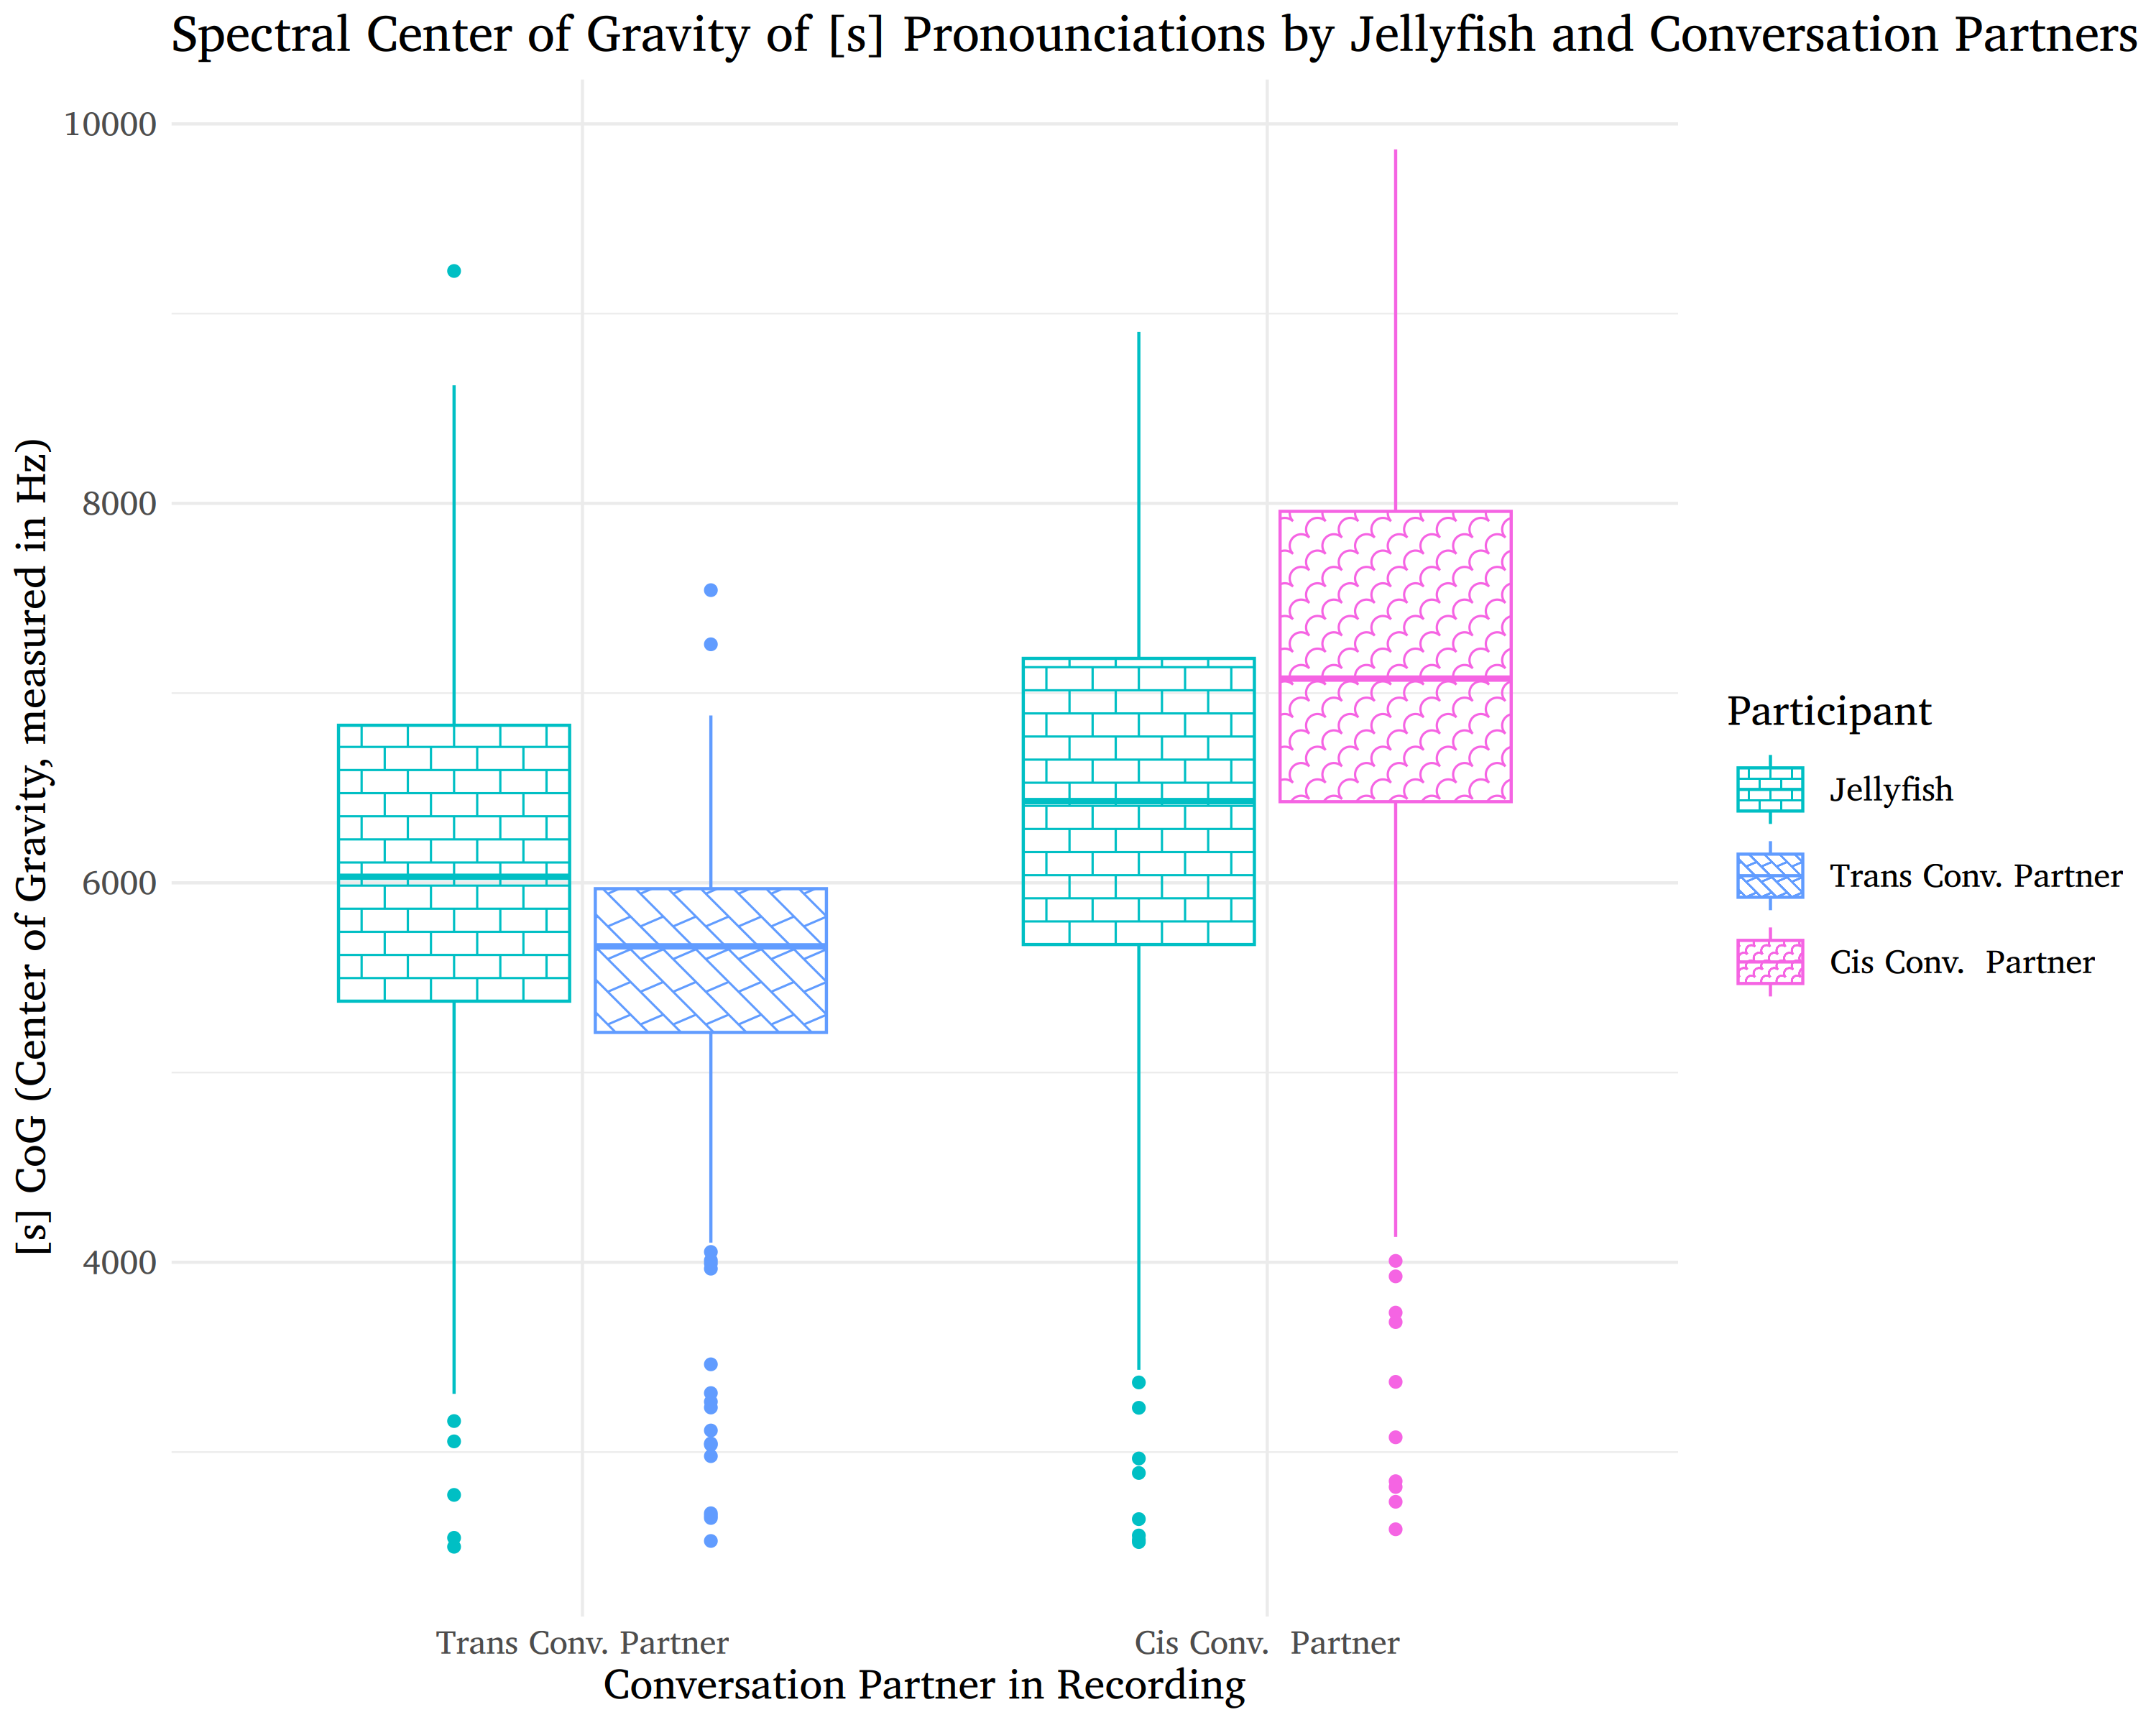
\includegraphics[width=\textwidth]{./images/Jellyfish _plot.png}
	\caption{CoG of /s/ pronunciations in each recording containing Jellyfish, her pronunciations and the pronunciations of the conversation partners.}
	\label{jellyfish_plot}
\end{figure}

Jellyfish, like Mantis, shifted towards fronter /s/ pronunciations when talking to the Cis CP, as shown in figure \ref{jellyfish_plot}. Unlike Mantis, Jellyfish's upwards shift is smaller, with a difference in mean CoG of ~300hz, and her overall mean CoG is lower, closer to Squirrel and Alpaca at 6154hz. In my interview with her, Jellyfish emphasized the importance of lesbianism to her identity and her relationship with her voice, saying that ``being a lesbian impacts the way that [she] move[s] through the world as a woman more than being trans does in a lot of situations,'' and that ``[she] can sound like a boy as a lesbian, with the way that [she] present[s], and have people just be like `oh that's like a weird dyke who smokes cigarettes','' which she considers to be an accurate description of herself. In this way, it makes sense to read her mean /s/ CoG as similar to that of the lesbian speakers \textcite{podesva_sexuality_2015} studied in Redding, California whose mean /s/ CoG was ~6300Hz.

Similar to Mantis, Jellyfish lays out her transition as a process of increasing confidence in her gender and increasing ability to resist or cast off hegemonic feminine norms. For Jellyfish, this takes the shape of the development of a lesbian boy identity against earlier internalizations of ideological transphobia. She notes:
\begin{quote}
 ``When I was in high school ... I would like look at all this like TERF\footnote{`TERF' is an acronym for `trans-exclusionary radical feminist', a label for a transphobic ideology which attempts to justify itself through appropriation of feminism.} propaganda and more or less like fashion myself to be the exception to like the narrative around trans people.''
\end{quote}
She later notes that this caused her to become ``kind of a psychopath, about like, presentation'', paying obsessive attention at that time to ``do like everything possible to fool people into thinking [she] was a cis woman''. This was also the period where she notes:
\begin{quote}
``I realized that women whistle on their `s's way more, and I remember like consciously changing how I speak to like whistle on the `s' more''
\end{quote}
This level of awareness of /s/ fronting is striking, and very interesting on its own. But even as an example of heightened awareness of hegemonic feminine norms and concern with having a `passing' voice, this can be read as providing evidence for my prediction that speakers who report greater pressure to conform and pass through their voice will shift to fronter /s/ with the Cis CP. However, it is important to note that Jellyfish situates this quite clearly as an aspect of her past more than her present.

By contrast, Jellyfish's present is much more characterized by an attitude of resistance towards rigid conformance to a singularly feminine gender and expression. She expresses this confidently:
\begin{quote}
`` I don't think it benefits me in any sort of way to like restrict myself like that... people are way to serious about all this shit, ... like, if I'm dressed more masculine in a certain day I'll like listen to different music and I'll like talk differently and I'll move differently and I just think that's fun!''
\end{quote}
When considered in light of my prediction that speakers who express attitudes of resistance towards hegemonic feminine norms will not shift to a fronter /s/ with the Cis CP, Jellyfish's outlook here perhaps raises the possibility a view of shifting to a fronter /s/ not as a conformist move towards the hegemonic norm, but rather as a shift in one's desired presentation to harmonize with those around her. This view is also supported by her comment that she ``"love/s/ talking like a boy when [she's] interacting with other boys''; this can be read as a form of harmonizing gender fluidity, which is certainly still resistance, but allows for shifting of /s/ frontness in the direction of one's listener's /s/ frontness.

In a similar way to Mantis, Jellyfish also serves as a counter-example against my prediction that speakers who expressed concern with misrecognition would not shift /s/. Her discussion of this concern provides additional insights. She presents the issue of `sounding like a gay guy' as particularly a concern in interaction with cis women, and something that sometimes will happen unconsciously, noting that:
\begin{quote}
 ``It is like, annoying at times when I like, default back to talking like a gay guy around cis women ... more than sounding like a boy sounding like a gay guy is like, terrifying, because there's this relationship that, it's mostly cis women, have with like trans women where you will be accepted and tolerated as like a gay guy but anything beyond that, if you like, don't know your place more or less, you're getting into dangerous territory.''
\end{quote}
Jellyfish clarifies here that `sounding like a gay guy' is not only a concern because of the inaccuracy and denial of her gender, but further that it represents a dangerous type of transphobia which hides itself behind a friendliness towards cisgender queer people. That she feels she might `default back to' speech she considers gay-male sounding around cis women may suggest a difficult and complicated process in which she subconsciously chooses to pursue the quasi-acceptance that gay men receive in spite of the invalidation of her gender and transphobia this comes along with. This may be able to explain, in part, why Mantis and Jellyfish shifted towards fronter /s/ pronunciations with the Cis CP, countering my prediction about speakers concerned with misrecognition.

%Learned a highly passing voice
%“It is like, annoying at times when I like, default back to talking like a gay guy around cis women”
%“you will be accepted and tolerated as like a gay guy but anything beyond that, … you're getting into dangerous territory”

\section{Speaker 2: Alpaca}
\begin{figure}[h]
	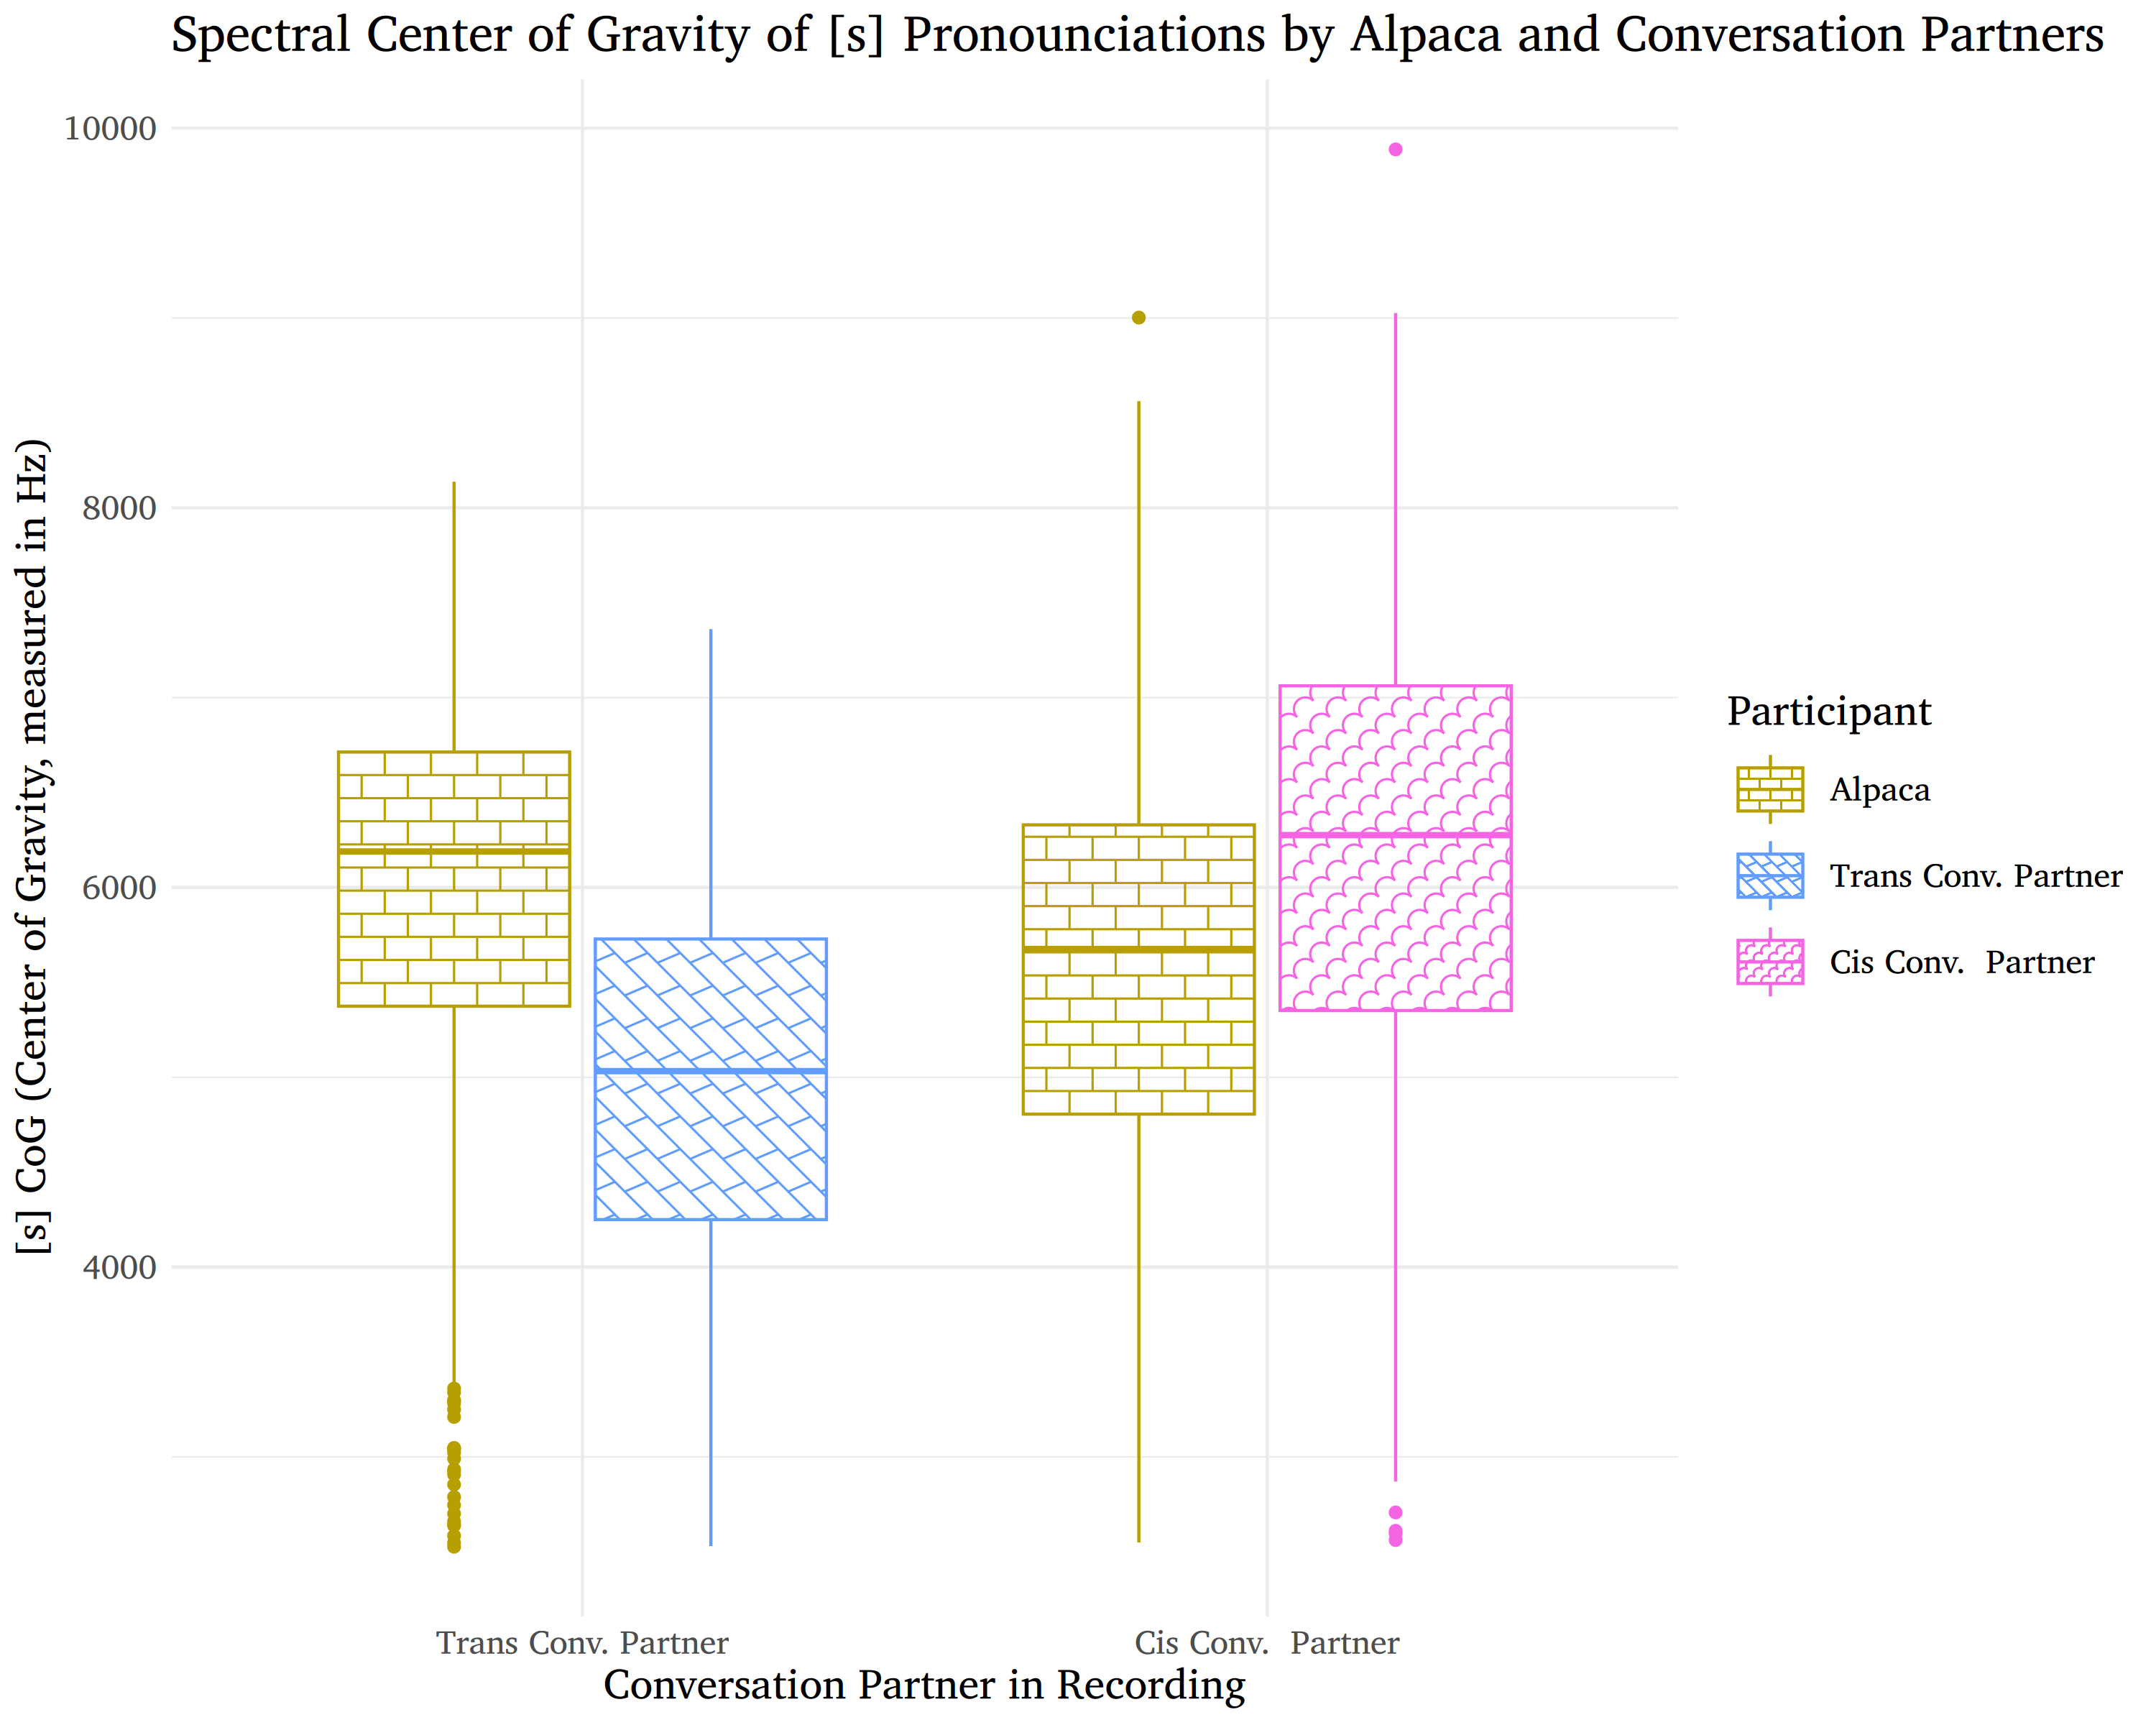
\includegraphics[width=\textwidth]{./images/Alpaca _plot.png}
	\caption{CoG of /s/ pronunciations in each recording containing Alpaca, her pronunciations and the pronunciations of the conversation partners.}
	\label{alpaca_plot}
\end{figure}

Alpaca's /s/ pronunciations are shown in \ref{alpaca_plot}. Alpaca differed from Mantis and Jellyfish firstly in that she shifted her /s/ pronunciations to be backer with the Cis CP, rather than fronter; her CoG reduces by ~400Hz. Also notable is that her overall average CoG of 5758Hz is the second lowest of my participants, only higher than the Trans CP's (5133Hz).

Also unlike Mantis and Jellyfish, Alpaca did not mention concern with sounding like a gay man in my interview with her. It is possible that her backer /s/ pronunciations are part of the reason that this concern does not come up for her, as her /s/ pronunciations are not front enough to trigger a misrecognizing gay-male indexicality. However, because this sort of misrecognition is not a concern for Alpaca, it also cannot easily be used to explain her shift to a backer pronunciation.

With respect to attitudes of resistance, the other factor my predictions associate with a lack of fronting around the Cis CP, Alpaca also differed from Mantis and Jellyfish. For Mantis and Jellyfish, the development of gender confidence involved a movement away from an initial feeling of pressure to strictly adhere to hegemonic femininity, and a gradual reclamation of behaviors which may hold hegemonic masculine associations as valid parts of a woman's identity. Alpaca describes the progression of her understanding of her gender differently:

\begin{quote}
``I think it's been a process of just sort of like getting more comfortable with femininity, because not wanting to be masculine, is, in my thought process, is kind of different from, ... coming to terms with the fact that I do like femininity and that I am comfortable with it and that it is something I can enjoy and be comfortable in and have as my own part of my identity ...''
\end{quote}

In this way, it seems that Alpaca's journey has been more of a gradual move towards comfort with elements of hegemonic femininity, rather than a gradual move towards accepting deviation from those norms. For this reason, Alpaca may feel less of a need to resist hegemonic femininity than Mantis and Jellyfish, as it may fall closer to a comfortable identity for her than it does for the prior two speakers. Under this interpretation, if Alpaca is not seen to hold a particularly strong attitude of resistance against hegemonic femininity, this also cannot explain her shift to backer /s/ pronunciations with the Cis CP.

With respect to the degree of concern with passing around cis people, it may be possible to argue that Alpaca was less concerned than Mantis and Jellyfish, partially explaining her lack of shifting. Unlike the prior two speakers, Alpaca does not bring up cis women's perceptions as dangerous or frustrating. Although she does note
\begin{quote}
 ``when I'm around other trans people I kind of feel less pressure ... to try to present perfectly femininely, like I feel less pressure to like pass ... in class or around cis people I might try to have a more feminine voice''
\end{quote}
Her stance seems to be more neutral than Mantis and Jellyfish, whose discussion of interacting with cis people contained more feelings of discomfort, danger, and dysphoria. Although it is of course possible that Alpaca does feel these ways and simply did not express it explicitly in the interview, it seems also possible that she is somewhat less concerned and this may have been responsible for her lack of shifting.

Alpaca also notes that she was not completely sure whether the Cis CP was cis. This was a result of my choice not to explicitly inform speakers of the trans status of the conversation partners, in order to reduce priming effects. Although she did suspect that the Cis CP may have been cis, she also believed it was possible that the Cis CP was a highly passing trans woman. As a possible confounding factor, this may also play a role in explaining Alpaca's difference in behavior from the other speakers.

%“I learned the exercise to raise your larynx”
%“I've just sort of subconsciously figured out how to use my voice in ways that sound more feminine”
%Does not mention ‘having gay voice’

\section{Speaker 3: Squirrel}
\begin{figure}[h]
	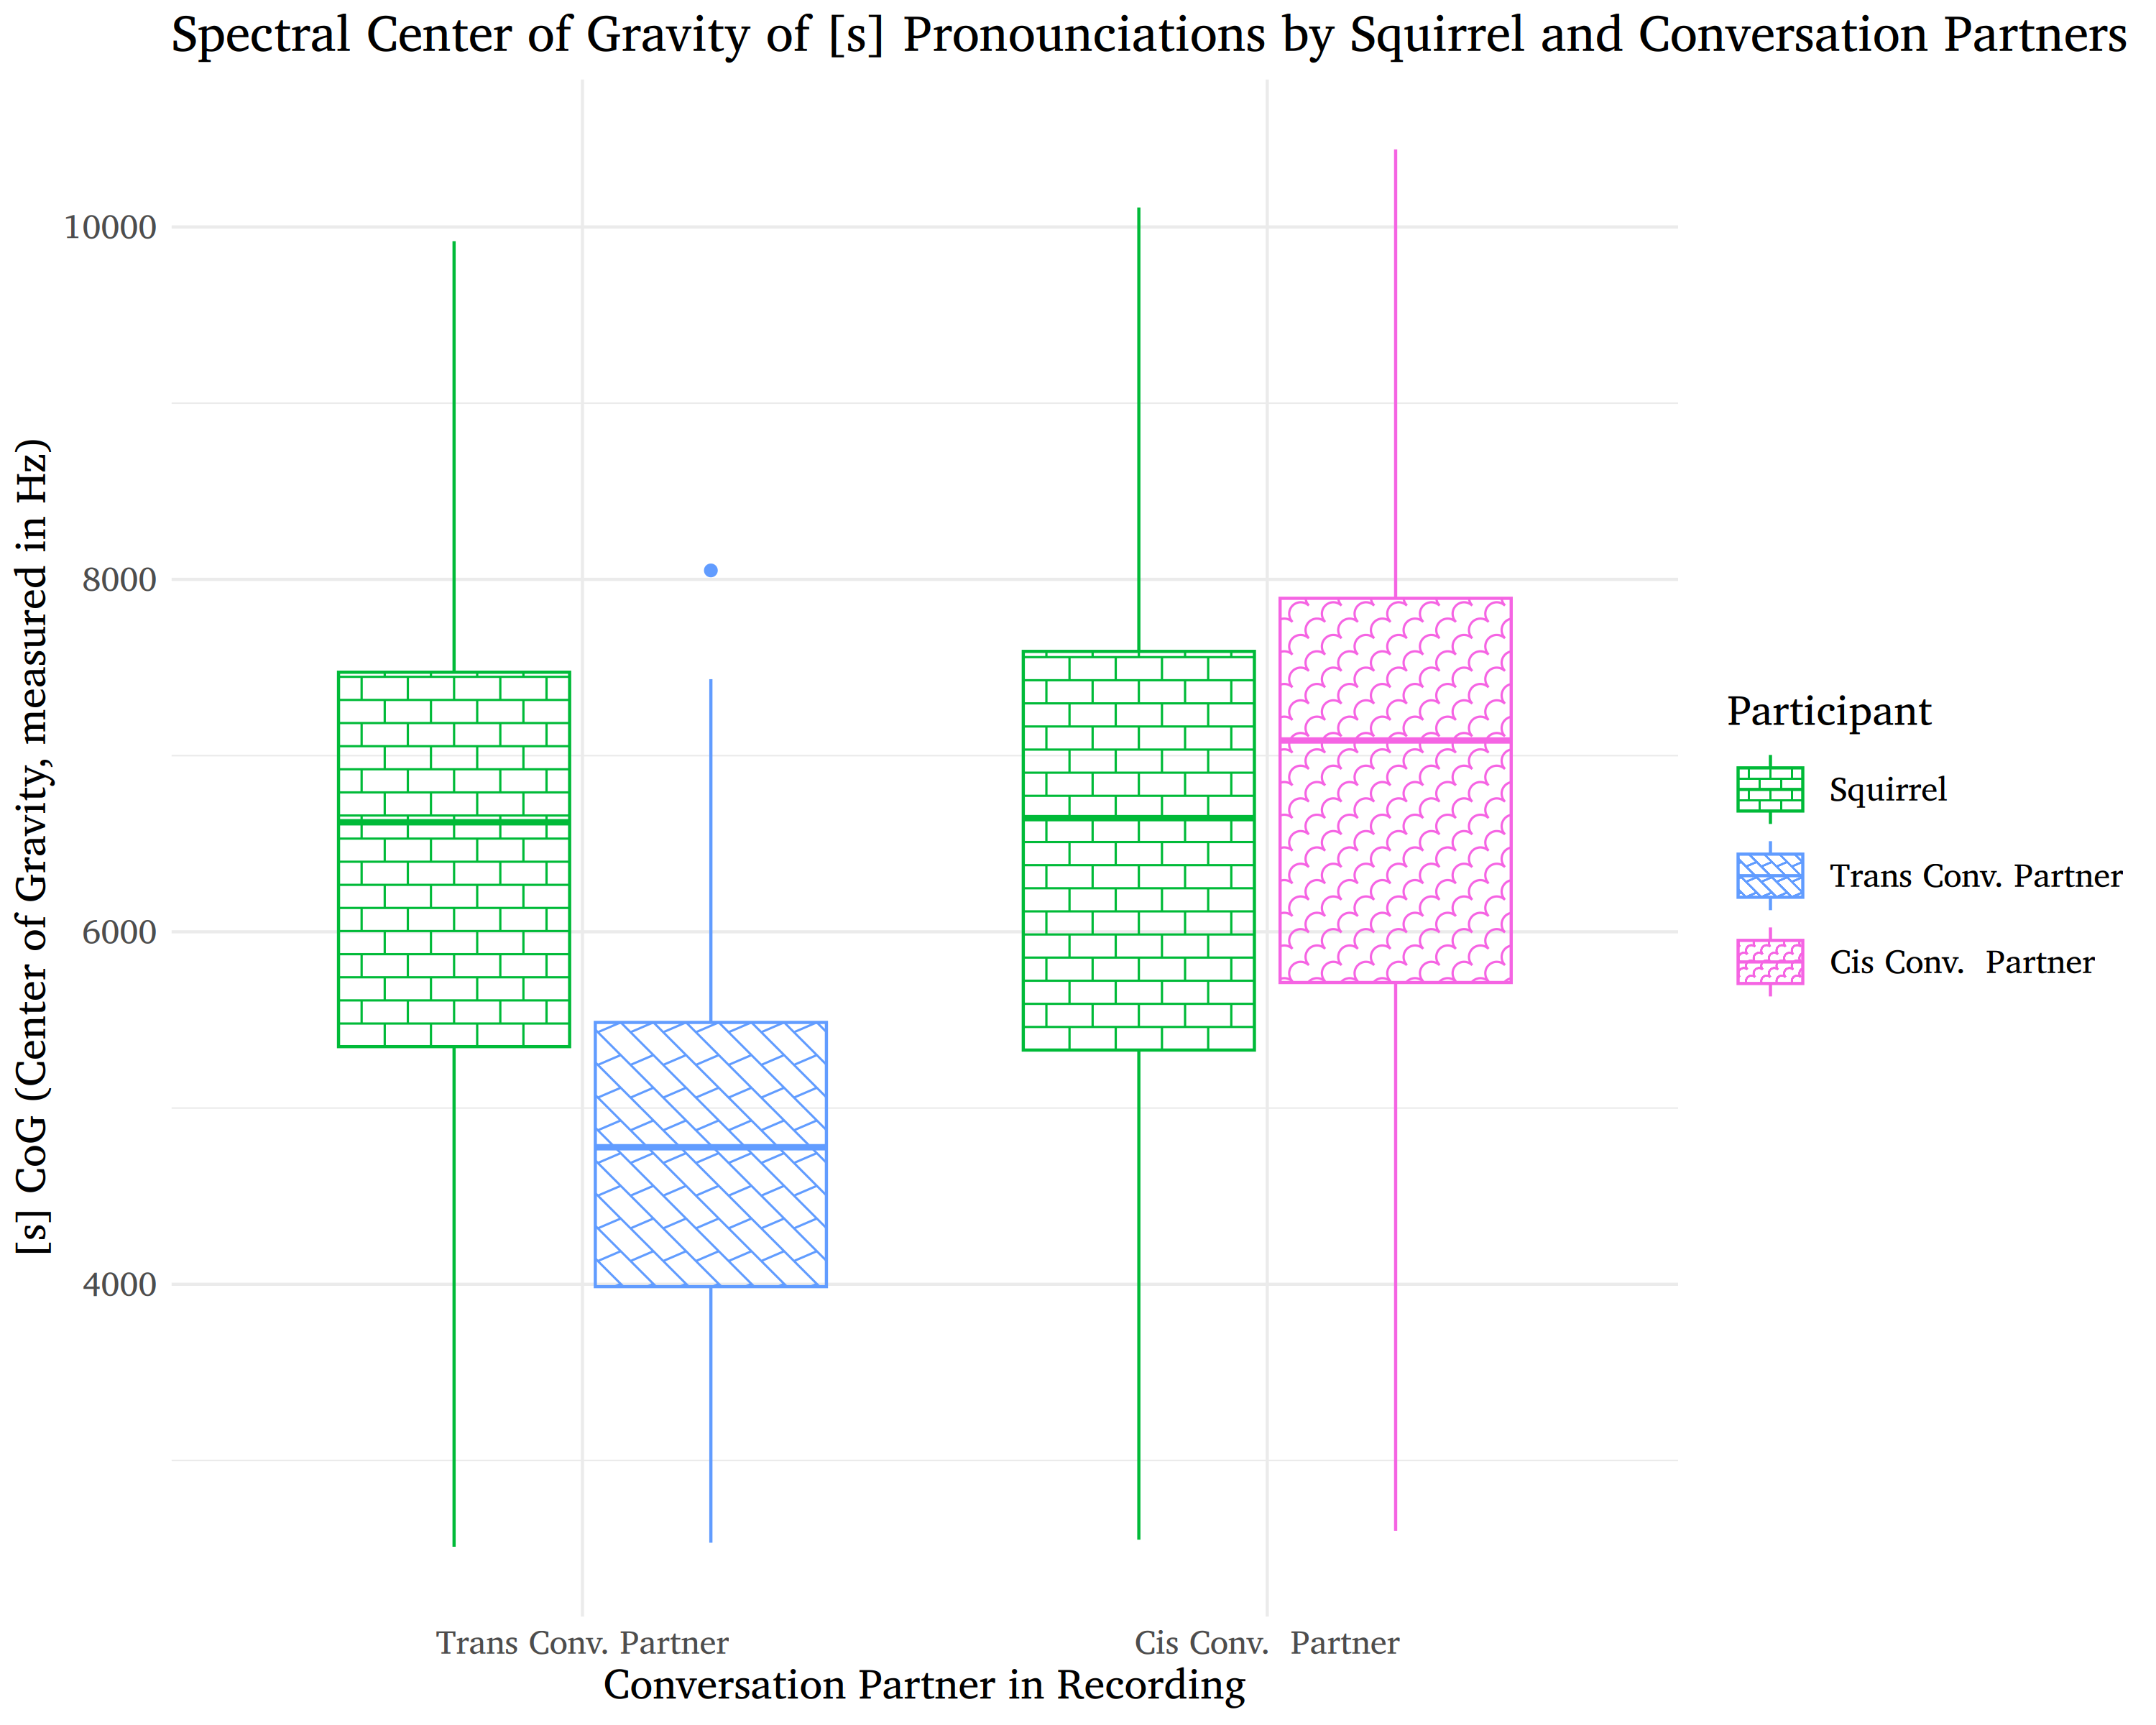
\includegraphics[width=\textwidth]{./images/Squirrel _plot.png}
	\caption{CoG of /s/ pronunciations in each recording containing Squirrel, her pronunciations and the pronunciations of the conversation partners.}
	\label{squirrel_plot}
\end{figure}

Squirrel stands out as the only speaker who did not shift her /s/ pronunciations, maintaining a CoG of ~6300Hz with both of the conversation partners (as shown in figure \ref{squirrel_plot}). She is also the only speaker in the early stages of her transition, having realized she was trans less than a year before the study, not yet having come out fully and beginning her social transition. In my interview with her, she explained that she ``didn't feel comfortable enough yet to'' take up a transfeminine presentation, and that she planned to progress in her physical transition through HRT and then take up her social transition in the following academic year, and that she planned to work on voice training in the summer before coming out. In light of this, it is perhaps surprising that her /s/ pronunciations are not backer, as she is the speaker participant with the second highest overall mean at 6357Hz. Although she had not yet begun efforts on voice training, it is possible she had already taken some less conscious steps towards a feminine voice, or that her /s/ pronunciation had already been in this range pre-transition. In the interview I asked her whether she felt that her voice was already feminine now, and she replied:
\begin{quote}
``that's a complicated question... sometimes, sometimes not... when I was really young ... I used to be really insecure about my voice, but for the opposite reason, that I thought it was like too fem.''
\end{quote}
Although she cites a high overall voice pitch as the primary cause for these pre-transition insecurities, it is possible that /s/ pronunciations similar to those used by queer women also played a role.

According to my predictions, speakers who hold greater attitudes of resistance towards hegemonic feminine norms and speakers who have concerns of misrecognition should be less likely to shift in /s/ pronunciations. From my interview with her, it seems that attitudes of resistance towards hegemonic feminine norms may be a factor in her choice not to shift working in combination with the potential lack of developed ability to shift as a result of transition stage. She notes that although she does intend to move towards a more feminine presentation,
\begin{quote}
``I think a lot of times there's like this expectation of if you're transfem that you're like hyper-fem and that's not how I feel really personally, like I don't know if `butch' is the right word for that but I definitely feel like the way that like I wanna present is not like super-hyper-fem''
\end{quote}
Similar to Mantis and Jellyfish, Squirrel affirms here that she does not want to and does not have to strictly follow hegemonic feminine norms, and that she hopes to inhabit a femininity which may contain elements hegemonically associated with masculinity. She explains this through clothing, mentioning that she would prefer to wear all-black than a brightly colored sundress.

It is notable that even though Squirrel's /s/ pronunciations are comparable to the /s/ pronunciations used by the gay men and trans women in Redding, California (a town likely similar to Squirrel's hometown, also in California) studied by  \textcite{podesva_sexuality_2015}, as she does not mention having concerns about being mistaken for a gay man with the sound of her voice. This may stand as a counterexample to the notion that the presence of these concerns apply to all transfem speakers with fronter /s/ pronunciations. It is sufficient to note here that this eliminates concern with misrecognition as an explanation for Squirrel's lack of shifting, counter to my predictions.

Squirrel's lack of shifting may also be interpreted as a counter-example to my prediction that speakers who expressed greater concern with sounding feminine and passing would be more likely to shift, as it seemed that this concern was quite present for her. When I asked her about her relationship with her voice, she begun by explaining that in online voice chat interactions,
\begin{quote}
``I like don't talk to a lot of people like that I would normally talk to if I was cis... as soon as I like basically came out to like my [online videogaming group]... I stopped talking entirely, on voice. ... I feel like it's easier for them to perceive me and like use correct pronouns like, if they don't hear me, because my, there's voice dysphoria, and like, my voice isn't like, they way I would want it to be if I could like pick it basically.''
\end{quote}
She explains further that
\begin{quote}
``I feel like inherently when like you hear someone for the first time you kind of assign like gender in your head to like that person... if you hear a stereotypically more masc voice then you might like automatically start like `he/him'ing someone in your head.''
\end{quote}
Here, she implicitly characterizes her voice in its current state as `stereotypically more masc', and that the best way to avoid being perceived as a man in online interactions with cisgender people is simply to not use her voice. For her, this falls under the general preference articulated as ``the more ways I can like not perceived, the better.'' In this context, it is perhaps understandable that pressure to pass does not lead to a shift in /s/, as Squirrel perceives a passing or feminine voice as not yet in reach at her current stage of transition, and thus does not have access to /s/ shifting.

\chapter{Discussion}

Based on the results above, it is clear that some transfeminine speakers do shift their /s/ pronunciations depending on the trans status of their listener. This provides an answer to the first and simplest research question of this thesis. This result -- the shifts exhibited by Mantis and Jellyfish to fronter /s/ pronunciations -- can be interpreted as evidence of the influence of the cisgender listening subject. In addition to its relevance to transfem thinking about the voice and being heard raised by \textcite{heffernan_constructing_2023} and its inhabitation by real cisgender listeners shown by \textcite{jessee_cisgender_2025}, it is clear that the presence of the cisgender listening subject does, for some speakers, impact actual linguistic behavior. This study thus supports the usefulness of listening subjects as a theorization of the mediation between perception of speech and production of speech, especially for trans speakers.

Central to this mediation is the question of how speakers' mental models of how their speech may be perceived inform their subsequent choices of linguistic variants. My results complicate this question; the relationships between the attitudes and concerns expressed in the interviews and observed behavior are mostly unexpected, and did not align with the model I initially constructed.
It is notable that even though all four speaker participants did express concerns about cisgender judgement and that they would change how they speak to be more feminine around cis listeners -- evidencing mental salience of the cisgender listening subject -- only two out of the four speakers implement this change in practice with /s/. Future research considering multiple linguistic features together could be especially illuminating here; it is possible that the Alpaca and Squirrel do also make changes towards more hegemonically feminine indexicalities with the cisgender listener, but that these changes are along features other than /s/, such as overall pitch (f0), intonation, voice quality, or discourse markers.

In the model I initially constructed, speakers who expressed greater degrees of struggling with voice dysphoria, greater desire have a voice which 'passes' as the voice of a cisgender woman, or a greater sense of danger and pressure to conform around cisgender listeners would be more likely to shift to a fronter /s/ pronunciation. On the other hand, speakers who expressed stronger attitudes of resistance against cisnormativity, differentiated themselves from hegemonic femininity, or were concerned that their voice might make them sound like a gay man would be more likely not to shift to a fronter /s/ pronunciation. In interpreting the explanatory failure of this model on my data, it is first important to note that its formulation tacitly constructs a mutual exclusivity of the former and latter concerns, which is not upheld by my data. Not only did Alpaca and Squirrel, who did not shift, express the factors I thought would predict no shift in /s/ less than Mantis and Jellyfish did, but further it seems that for Mantis and Jellyfish, the former concerns (which I thought would predict a shift to fronter /s/) are caused by the latter concerns (which I thought would predict no shift).

The issue of misrecognition is central here. In Mantis' discussion of how her voice is percieved, sounding like a straight man is not considered a possibility; if she is perceived correctly she will sound like a queer woman, and if she is perceived incorrectly she will sound like a gay man. Within the model of /s/ indexicality brought forth by \textcite{calder_sissy_2019} (recall figure \ref{figure_fractal_recursivity_indexical_orders}), other semiotic information is used to determine through which indexical order /s/ pronunciations will be interpreted. From this perspective, a shift in /s/ pronunciations could be considered useless for Mantis, in that whether she will be heard as a gay man or a cis woman cannot be determined by her /s/ pronunciation. Yet she shifts, contradicting the model. The extent of her shift provides help here; she shifts to /s/ pronunciations which fall in closer line with those expected of cis women than those reported for cis gay men. Within the literature reviewed, \textcite{zimman_hegemonic_2013} gives the highest mean CoG for cisgender gay men (not in drag) in the literature reviewed at ~6550Hz, whereas Mantis' /s/ pronunciations with the Cis CP had a mean CoG of 7964Hz, well within the hegemonically expected range of cis women. In \textcite{calder_sissy_2019}, SoMa queens front /s/ further than Castro queens in order to forge a higher indexical order and index a radical queer femininity beyond mainstream cisgender gay male femininity. Here, I argue that Mantis fronts /s/ further than cis gay men do, but that no higher order of indexicality can be forged, as she must make do with the two hegemonic indexical orders already existing in the indexical inventory of her listener; instead, she uses this much more fronted hegemonically-feminine /s/ access to the lower level of indexicality and encourages her /s/ pronunciations to be interpreted as those of a woman on the $n$th level, and not those of a gay man on the $n + 1st$.

Although this extension of the model works for Mantis, the situation is different for Jellyfish. If it is indeed the case, as Jellyfish mentions, that ``when you're a lesbian sounding like a gay guy and like having a faggcent will get you clocked way more than sounding like boy,'' why does she choose to shift to a fronter /s/ rather than not shifting /s/ and 'sounding like a boy'? Although it is not easy to answer this question with certainty from the data available and without context of other indexical features, I see three possible explanations. First, it is possible that Jellyfish is simply mirroring the /s/ pronunciations of her CPs, and that questions of perception of gender and sexuality are less relevant to this case. A point in favor of this explanation is the priority Jellyfish lends to her lesbian identity; because the Cis CP was also a lesbian, it is possible that the function of linguistic mirroring in this case could have been a move to create greater similarity between herself and her CP, a move of `adequation' from the perspective of the `tactics of intersubjectivity` theorized by \textcite{irvine_language_2000}. The second possible explanation has to do with the complexity of Jellyfish's relationship with expressing boyness. Although she indicates that it is at least hypothetically safer for her to sound like a boy than a gay man around cis women, she also clarifies that ``I'm like less concerned about like trying to like overly feminize my voice when I'm around other trans people'', and that ``I love talking like a boy when I'm interacting with other boys''. From this perspective, it is possible that she felt less comfortable to sound like a boy with the Cis CP, and thus ``with like, it's mostly people I don't know, I'll like try harder to um have like a more conventionally feminine voice.'' A point of dissatisfaction with this second explanation is that it breaks down when considered for the other speakers; as mentioned above, all speakers indicated similar sentiments that they would shift towards hegemonically feminine speech with cisgender listeners, but Alpaca and Squirrel do not in fact shift /s/ in this way. The third, and perhaps more promisingly generalizable, explanation for Jellyfish's shift has to do with agency and the notion of a `natural' voice. In her discussion of her concerns with misrecognition, she underlines that although she is proud of ``being able to more or less manipulate [her voice] how [she] want[s]'', she nonetheless is sometimes bothered that she might
\begin{quote}
``default back to talking like a gay guy around cis women ... It's kind of rolling the dice what voice comes out on a certain day, and sometimes the faggcent comes back''
\end{quote}
Her notion that a voice more prone to misrecognition (`the faggcent') is a `default' for her around cis women and her metaphor of styleshifting to rolling dice make it clear that she does not feel fully in control of her voice. Here, it is possible to understand her shift to a fronter /s/ pronunciation with the Cis CP as an example of this sort of `defaulting', rather than an agentive choice aligned with her intentions and goals. It is further interesting that in her discussion of how she talks around other trans people, comfort in her voice is also described in terms of defaulting:
\begin{quote}
``at a certain point, I like stop performing and sort of default back to like my neutral state which is still just like talking like a boy, which is fine, like I don't really feel much pressure to change that.''
\end{quote}
Although Jellyfish does acknowledge that ``it's all performance'', in line with feminist understandings of gender performativity, it is nonetheless notable that Jellyfish perhaps considers hegemonic femininity somewhat of a difficult or unnatural performance for her, and that it does not feel like her neutral state. Here, it is clear that styleshifting is not effortless, always available, and without cost; instead, it comes to be limited.

From this, I am motivated to take up the question of the interplay between agency and limits on agency as central to the interpretation of my data. In the introduction to this thesis, I mentioned that agentic models of linguistic variation, which see speakers' linguistic practices as strategically and intentionally deployed to achieve social goals, was limited by the restrictions imposed by the importance of the listener's role in interpretation. From my results, it seems additionally important to consider the degree to which variants are available and natural to speakers; even if a speaker's vocal tract holds the potential to produce a wide degree of linguistic variants, it is nonetheless possible that a speaker may only be familiar with using only a smaller range of variants, or experience some variants as more effortful and less natural due to their varying familiarity. An analogy can be made to phonology in language learning; it is an uncontroversial fact of language that all humans with typical vocal tracts are capable of all phonetic and phonemic distinctions in all human languages, but it is also uncontroversial that learning the phonology of a new language is challenging and time-consuming, and that effort is required to sustain accurate pronunciation.

I argue that this framework of limited agency helps explain Alpaca and Squirrel's lack of normative shifting as well. For Squirrel, the reasoning is fairly simple; as a transfem early in the process of transition, Squirrel considers a feminized voice as only accessible in the future. The inaccessibility of her desired voice -- her voice not being ``they way [she] would want it to be if [she] could like, pick it'' -- is complete enough that she does not use her voice at all on the internet, the sphere in which she wishes to be perceived as feminine. Being not fully out in in-person interactions means that she is for the time being continuing to assume she might be perceived as masculine, and does not yet feel able to combat these perceptions through the voice.

For Alpaca, I believe that this framework can help explain her lack of a frontwards shift, although the backwards directionality of her shift remains difficult to explain. Alpaca mentions learning ``the exercise to raise your larynx'', and has the sense that she has implemented this into her everyday speech over the course of her transition, noting that she ``learned how to do it and then [she] found [her]self sort of subconsciously doing it'' over time. The status of agency in this example is instructive to unpack; despite the ability to raise the larynx always existing in her vocal tract, learning the exercise she mentions provides a greater degree of access to this variant. That she found herself ``subconsciously doing it'' indicates another complex relationship with agency, whereby changes could not be forced but become more natural and less effortful over time. With respect to /s/, it is possible that this resource for gendered indexicality is not easily accessible for Alpaca, and perhaps feels less needed in the context of her perceived success in feminizing her voice over the years of her transition. Because shifting /s/ fronter would require accessibility and effort, this change is not made. That this cannot account for why Alpaca shifts to backer /s/ pronunciations is not ideal, but perhaps not a problem for the framework; there do not seem to be any factors found in Alpaca's identity or interview which could be used to explain the directionality of her shift, so it is likely that more data would be needed to resolve this issue.

It is also important to clarify that this framework of limitations on agency certainly does not imply that all of my speakers' behavior can only be explained by limitations rather than agentivity. As discussed above, I argue that Mantis represents an example of agency as a better explanation than limitation, in that her shift is the most drastic, and it simultaneously achieves both of her goals; to protect herself from dysphoria and negative judgment by her listener by taking up fronted /s/ as a hegemonically feminine index, and to protect herself from gay-male misrecognition by using fronter /s/ pronunciations than would be expected from gay men. My first possible explanation of Jellyfish's behavior may also suggest agency as a primary explanatory frame. These sorts of goal-satisfying use of linguistic resources is unproblematically read as agentive, even though it is defensive in Mantis' case. My argument here is for the both-and of agentivity and limitation, seeing that my data is best explained when both considerations are given weight and relevance. After all, this model more suitably describes the social world my participants live within; they are limited by their societies and their abilites, but nonetheless can agentically and strategically make choices when those choices are accessible and intentionally available.

% affective mediating layers / talk about ``customer service voice'' as ``not even an intentional gender thing''?


\chapter*{Conclusion}
         \addcontentsline{toc}{chapter}{Conclusion}
	\chaptermark{Conclusion}
	\markboth{Conclusion}{Conclusion}
	\setcounter{chapter}{5}
%	\setcounter{section}{0}

In conducting an initial investigation transfeminine speakers' negotiation of cisheteronormativity through the use of the /s/ sound, this thesis aims to shed light on the uneasy interplay of the limitations that power structures impose and the agency individuals have to resist those norms. Research on trans speech has primarily placed its focus on one or the other side of this contrast. When speakers are investigated in only one context, whether it be a safe queer space, or a possibly-unsafe cisgender space, the contrasting influences of safety and conformity on behavior cannot be seen clearly. As a particularly complex site of gendered speech performativity, fronting /s/ is a difficult choice for transfems; on the one hand, survival within the cisgender world is often difficult and requires conformity, but on the other, conformance requires effort, is not always readily available even if physically possible, and should be resisted. Furthermore, even if a speaker does set out to conform to the hegemonic expectations of feminine speech by fronting /s/, it is not guaranteed that this will gain them the acceptance they seek; the risk remains that a cisgender listener may (intentionally or otherwise) misrecognize this index to signal a gay-masculine identity. In this way, they accept queerness but reject transness, protecting themselves in the comfortable misperception of transfeminine people as cisgender gay men.

The difficulty of sociolinguistic decisions is underlined by the unexpected correspondences between my speakers' /s/ shifting behavior and their expressed attitudes. The particularly vexing conflict between the indexical orders of /s/ and the threat of misrecognition this produces for transfeminine speakers attests to the analytic value of misrecognition as theorized by \cite{barrett_sexuality_2024} as a framework to understand the interaction of power structures and everyday behavior. Traditional sociolinguistic frameworks would predict that speakers who wished to differentiate themselves from hegemonic norms and present their desired identity would simply do so, where my data shows that this ability is sometimes stripped from speakers, who may have to prioritize their own feelings of safety and comfort over their identitymaking goals, or who may lack knowledge or practice with the indexical materials they would need to do so.

In proposing a nuanced approach to sociolinguistic decisions, this thesis does not intend to argue that marginalized speakers are stripped of agency and have no choice about how they present their voice, simply following norms to the extent they are able. This approach would fly in the face of the decades of sociolinguistic research which have worked to uncover the agentic freedom that linguistic variation offers in allowing speakers to present themselves and their voices in line with their social goals. Instead, I argue that agentic goals and limiting restrictions are always simultaneously present, and speakers, especially marginalized speakers such as transfeminine people, make difficult decisions in consideration of all of the factors. Importantly, speakers can tip the scales in the favor of agentivity if they are empowered with semiotic self-awareness; as my participant Jellyfish says,
\begin{quote}
``People take this shit way too seriously ... Fundamentally, queerness should change how you move through the world. I think that's a good thing, I think like having control of how you're perceived and how you interact with the world and thinking about that more is something that everyone should do, and my transness and my lesbianism are like vectors to which I do that.''
\end{quote}

	
\section{Limitations and Directions for Future Research}
A primary limitation of this study is its lack of a raciolinguistically informed approach. As a white researcher working with mostly white participants and drawing on a mostly white-centric research literature, I do not aim for this study to perpetuate the whiteness of trans studies, queer studies, and sociolinguistics. Research on BIPoC transfems' /s/ pronunciations on their own terms and in their own spaces would be highly illuminating. \textcite{calder_whose_2022} find that a gender split in /s/ pronunciation is not present for Black speakers in Bakersfield, California. If a study like this one were conducted with Black transfeminine speakers, it is possible that race of the perceiver may emerge as equally relevant as cisgender status, and that the influence of the white cisgender listening subject would exert multiplicative oppressive effects, an example of sociolinguistic intersectionality (see \cite{miles-hercules_real_2022}). Due to the dearth of research on Asian-Americans in the sociolinguistic literature, and the absence of research on Asian-American /s/ pronunciation, %TODO fact check this
It was regrettably difficult for me to determine the extent to which the whiteness of the hegemonic gendered expectations of /s/ frontness impacted the Asian-American speakers in my study, Mantis and the Trans CP. I encourage further research outside white speaker and perceiver populations, and hope to be able to work with queer and trans BIPoC sociolinguists and speakers to focus closer on race in the future.

Other limitations of this study pertain to scale and scope. As mentioned in my discussion, this study could greatly benefit from more angles of analysis in several ways. To name two, expanding to include multiple linguistic variables alongside /s/ would provide much-needed context and insights, and zooming in to the discourse level to inspect how /s/ was shifted within each individual conversation based on topic, stance, and mood would allow a more nuanced understanding of the moment-to-moment meaning-in-context of /s/ as it develops and shifts in conversation with the aggregated understanding I present. Further research would also benefit significantly from a larger scale, at which a greater diversity of participants and conversation partners could reveal broader patterns and reduce the possible confounds introduced by any idiosyncrasies of the individual personalities of the two conversation partners I have. This would also allow for a quantitative analysis of predictive factors of /s/ shifting, operationalizing with more precision the attitudes, concerns, and identities I consider qualitatively here.


%If you feel it necessary to include an appendix, it goes here.
    \appendix
      \chapter{Survey} \label{appendix_a}
      \chapter{Interview Questions} \label{appendix_b}


%This is where endnotes are supposed to go, if you have them.
%I have no idea how endnotes work with LaTeX.

  \backmatter % backmatter makes the index and bibliography appear properly in the t.o.c...

% if you're using bibtex, the next line forces every entry in the bibtex file to be included
% in your bibliography, regardless of whether or not you've cited it in the thesis.
    \nocite{*}

% Rename my bibliography to be called "Works Cited" and not "References" or ``Bibliography''
\renewcommand{\bibname}{References}

%    \bibliographystyle{bsts/mla-good} % there are a variety of styles available; 
%  \bibliographystyle{plainnat}
% replace ``plainnat'' with the style of choice. You can refer to files in the bsts or APA 
% subfolder, e.g. 
   % or
 \printbibliography
 % Comment the above two lines and uncomment the next line to use biblatex-chicago.
 %\printbibliography[heading=bibintoc]

% Finally, an index would go here... but it is also optional.
\end{document}
